\documentclass[a4paper]{report}
%----------japanese text command----------%
\newcommand{\jp}[1]{\begin{CJK}{UTF8}{min}#1\end{CJK}} 

%----------items----------%
\newcommand{\potion}[1][]{Potion #1(\jp{ポーション})}
\newcommand{\hiPotion}[1][]{HiPotion #1(\jp{ハイポーション})}
\newcommand{\phoenixDown}[1][]{Phoenix Down #1(\jp{フェニックスの尾})}
\newcommand{\revivify}[1][]{Revivify #1(\jp{せいすい})}
\newcommand{\maidensKiss}[1][]{Maiden's Kiss #1(\jp{おとめのキッス})}
\newcommand{\eyedrop}[1][]{Eyedrop #1(\jp{めぐすり})}
\newcommand{\antidote}[1][]{Antidote #1(\jp{どくけし})}
\newcommand{\tent}[1][]{Tent #1(\jp{テント})}
\newcommand{\flameScroll}[1][]{Flame Scroll #1(\jp{かとんのじゅつ})}
\newcommand{\elixir}[1][]{Elixir #1(\jp{エリクサー})}
\newcommand{\waterScroll}[1][]{Water Scroll #1(\jp{すいとんのじゅつ})}
\newcommand{\thunderScroll}[1][]{Thunder Scroll #1(\jp{らいじんのじゅつ})}
\newcommand{\cottage}[1][]{Cottage #1(\jp{コテージ})}
\newcommand{\ether}[1][]{Ether #1(\jp{エーテル})}
\newcommand{\speedDrink}[1][]{Speed Drink #1(\jp{スピードドリンク})}
\newcommand{\heroDrink}[1][]{Hero Drink #1(\jp{えいゆうのくすり})}
\newcommand{\turtleShell}[1][]{Turtle Shell #1(\jp{かめのこうら})}
\newcommand{\dragonFang}[1][]{Dragon Fang #1(\jp{りゅうのきぼ})}

%----------spells----------%
\newcommand{\life}[1][]{Life #1(\jp{レイズ})}
\newcommand{\fire}[1][]{Fire #1(\jp{ファイア})}
\newcommand{\bolt}[1][]{Bolt #1(\jp{サンダー})}
\newcommand{\cure}[1][]{Cure #1(\jp{ケアル})}
\newcommand{\goblinPunch}[1][]{Goblin Punch #1(\jp{ゴブリンパンチ})}
\newcommand{\exit}[1][]{Exit #1(\jp{テレポ})}
\newcommand{\reset}[1][]{Reset #1(\jp{リターン})}
\newcommand{\breakSpell}[1][]{Break #1(\jp{ブレイク})} 
\newcommand{\ltwoOld}[1][]{L.2 Old #1(\jp{レベル2オールド})} 
\newcommand{\lfiveDeath}[1][]{L.5 Death #1(\jp{レベル5デス})} 
\newcommand{\size}[1][]{Size #1(\jp{ミニマム})}
\newcommand{\float}[1][]{Float #1(\jp{レビテト})}
\newcommand{\reflect}[1][]{Reflect #1(\jp{リフレク})}
\newcommand{\haste}[1][]{ヘイスト #1(\jp{リフレク})}

%----------abilities----------%
\newcommand{\gilToss}[1][]{Gil Toss #1(\jp{ぜになげ})}
\newcommand{\cover}[1][]{Cover #1(\jp{かぼう})}
\newcommand{\combine}[1][]{Combine #1(\jp{ちょうごう})}
\newcommand{\black}[1][]{Black #1(\jp{くろまほう})} 
\newcommand{\blue}[1][]{Blue #1(\jp{あおまほう})} 
\newcommand{\magicSword}[1][]{Magic Sword #1(\jp{まほうけん})} 
\newcommand{\kick}[1][]{Kick #1(\jp{けり})} 
\newcommand{\guard}[1][]{Guard #1(\jp{まもる})}
\newcommand{\steal}[1][]{Steal #1(\jp{盗む})}
\newcommand{\throw}[1][]{Throw #1(\jp{なげる})}
\newcommand{\catch}[1][]{Catch #1(\jp{とらえる})}
\newcommand{\observe}[1][]{Observe #1(\jp{しらべる})}
\newcommand{\release}[1][]{Release #1(\jp{はなつ})}
\newcommand{\white}[1][]{White #1(\jp{しろまほう})} 
\newcommand{\escape}[1][]{Escape #1(\jp{とんずら})} 
\newcommand{\tame}[1][]{Tame #1(\jp{なだめる})} 
\newcommand{\gaia}[1][]{Gaia #1(\jp{ちけい})} 
\newcommand{\hide}[1][]{Hide #1(\jp{かくねる})} 
\newcommand{\drink}[1][]{Drink #1(\jp{のむ})} 
\newcommand{\dash}[1][]{Dash #1(\jp{ダッシュ})} 
\newcommand{\learning}[1][]{Learning #1(\jp{ラーニング})} 
\newcommand{\control}[1][]{Control #1(\jp{あやつる})} 
\newcommand{\dimenAbility}[1][]{Dimen #1(\jp{じくう})} 
\newcommand{\showAbility}[1][]{Show #1(\jp{あらねれる})} 

%----------weapons----------%
\newcommand{\broadsword}[1][]{Broadsword #1(\jp{ブロードソード})}
\newcommand{\knife}[1][]{Knife #1(\jp{ナイフ})}
\newcommand{\daggerWeapon}[1][]{Dagger #1(\jp{ダガー})}
\newcommand{\iceRod}[1][]{Ice Rod #1(\jp{こおりのロッド})}
\newcommand{\mythrilKnife}[1][]{Mythril Knife #1(\jp{ミスリルナイフ})}
\newcommand{\fireRod}[1][]{Fire Rod #1(\jp{ほのおのロッド})}
\newcommand{\thunderRod}[1][]{Thunder Rod #1(\jp{いかづのロッド})}
\newcommand{\kunai}[1][]{Kunai #1(\jp{くない})}
\newcommand{\shuriken}[1][]{Shuriken #1(\jp{しゅりけん})}
\newcommand{\ancientSword}[1][]{Ancient Sword #1(\jp{こだいのつるぎ})}
\newcommand{\dancingDagger}[1][]{Dancing Dagger #1(\jp{ダンシングダガー})}
\newcommand{\airBlade}[1][]{Air Blade #1(\jp{かぜきりのやいば})}

%----------armor----------%
\newcommand{\crystalShield}[1][]{Crystal Shield #1(\jp{クリスタルのたて})}
\newcommand{\silkRobe}[1][]{Silk Robe #1(\jp{シルクのローブ})}
\newcommand{\stealthRobe}[1][]{Stealth Robe #1(\jp{しのびのころも})}
\newcommand{\goldArmor}[1][]{Gold Armor #1(\jp{ゴールドアーマー})}
\newcommand{\iceBow}[1][]{Ice Bow #1(\jp{こおりのゅみや})}
\newcommand{\powerWrist}[1][]{Power Wrist #1(\jp{パワーリスト})}
\newcommand{\greenBeret}[1][]{Green Beret #1(\jp{グリーンベレー})}
\newcommand{\goldShield}[1][]{Gold Shield #1(\jp{ゴールドシールド})}
\newcommand{\boneMail}[1][]{Bone Mail #1(\jp{ボーンメイル})}
\newcommand{\iceShield}[1][]{Ice Shield #1(\jp{アイスシールド})}
\newcommand{\ribbon}[1][]{Ribbon #1(\jp{リボン})}

%----------accessories----------%
\newcommand{\runningShoes}[1][]{Running Shoes #1(\jp{エルメスのくつ})}
 
%----------misc----------%
\newcommand{\activeOption}[1][]{Active #1(\jp{アクティヴ})}
\newcommand{\shortOption}[1][]{Short #1(\jp{たんしゆく})}
\newcommand{\memoryOption}[1][]{Memory #1(\jp{きおく})}
\newcommand{\emptyOption}[1][]{Empty #1(\jp{すべてはずす})}
\usepackage[group-separator={,},group-minimum-digits={3}]{siunitx}
\usepackage[utf8]{inputenc}
\usepackage[dvipsnames]{xcolor}
\usepackage{tcolorbox}
\usepackage[margin=0.2in, paperwidth=12in]{geometry}
\usepackage{setspace}
\usepackage{hyperref}
\usepackage{titlepic}
\usepackage{CJKutf8}
\usepackage{soulutf8}
\usepackage{varwidth}
\usepackage{tocloft}
\usepackage{paracol}
\usepackage{tabu}

%----------page setup----------%
\definecolor{pageColor}{RGB}{240, 240, 240}
\pagecolor{pageColor}
\setlength{\columnsep}{.5cm}
\hfuzz=49pt 

%----------chapter setup----------%
\makeatletter
\def\@makechapterhead#1{%
  {\parindent \z@ \normalfont
    \ifnum \c@secnumdepth >\m@ne
        \huge\bfseries #1
        \par\nobreak
        \rule{\columnwidth}{.1pt}%
    \fi
    \interlinepenalty\@M
  }}
\makeatother

%----------hyperlinks----------%
\hypersetup{
    colorlinks,
    citecolor=black,
    filecolor=black,
    linkcolor=black,
    urlcolor=black
}

%----------misc setup----------%
\usepackage{enumitem}
\setitemize{noitemsep,topsep=0pt,parsep=0pt,partopsep=0pt}
\usepackage{graphicx}

\pagenumbering{gobble}
\setlength{\columnsep}{1.5cm}
\setlength{\columnseprule}{0.2pt}

\makeatletter
\patchcmd{\chapter}{\if@openright\cleardoublepage\else\clearpage\fi}{}{}{}
\makeatother

\DeclareUnicodeCharacter{2194}{\ensuremath{\leftrightarrow}}

%---------toc--------------%
\setlength{\cftbeforetoctitleskip}{-3.5mm}
\renewcommand{\cfttoctitlefont}{\Huge\bfseries}
\renewcommand{\cftaftertoctitle}{\par\nobreak\rule{\columnwidth}{.1pt}}

%----------style overrides----------%
\renewcommand{\theenumi}{\textbf{\arabic{enumi}}}
\renewcommand{\labelitemi}{$\bullet$}
\renewcommand{\labelitemii}{$\circ$}
\renewcommand{\labelitemiii}{$\ast$}
\renewcommand{\labelitemiv}{$-$}
\renewcommand{\familydefault}{\sfdefault}

%----------convenience commands----------%
\newcommand{\varwb}{\begin{varwidth}{\textwidth}}
\newcommand{\varwe}{\end{varwidth}}
\newcommand{\resume}{\vspace{-1pc}}
\newcommand{\alignBoxes}{\vspace{1.05mm}}
\newcommand{\switchcolumnTwice}[1][]{\switchcolumn\switchcolumn#1}
\newcommand{\insertScreenshot}[1]{\includegraphics[scale=0.3]{#1}}
\newcommand{\insertPath}[1]{\includegraphics[scale=0.5]{#1}}
\newcommand{\insertMap}[1]{\includegraphics[scale=1.1]{#1}}

%----------arrows and symbols----------%
\newcommand{\pointUp}{\textbf{↑}}
\newcommand{\pointDown}{\textbf{↓}}
\newcommand{\pointLeft}{\textbf{←}}
\newcommand{\pointRight}{\textbf{→}}
\newcommand{\switch}{\textbf{↔}}

%----------base colors----------%
\definecolor{red}{RGB}{234, 52, 35}
\definecolor{blue}{RGB}{47, 152, 222}
\definecolor{purple}{RGB}{139, 70, 229}
\definecolor{pink}{RGB}{235, 18, 127}
\definecolor{orange}{RGB}{245, 122, 0}
\definecolor{green}{RGB}{0, 181, 133}
\definecolor{yellow}{RGB}{253, 255, 84}

%----------colorbox colors----------%
\definecolor{menu}{RGB}{72, 188, 72}
\colorlet{menuHl}{menu!75}
\colorlet{menuHlTwo}{menu!65>wheel,1,2}
\definecolor{shop}{RGB}{228, 162, 9}
\colorlet{shopHl}{shop!70}
\colorlet{shopHlTwo}{shop!50>wheel,1,2}
\colorlet{shopHlThree}{shop!40>twheel,1,2}
\definecolor{boss}{RGB}{229, 51, 51}
\colorlet{bossHl}{boss!65}
\colorlet{bossHlTwo}{boss!65>wheel,1,2}
\colorlet{bossHlThree}{boss!70>twheel,1,2}
\definecolor{trainer}{RGB}{223, 113, 168}
\colorlet{trainerHl}{trainer!75}
\colorlet{trainerHlTwo}{trainer!90>wheel,1,2}
\colorlet{trainerHlThree}{trainer!95>twheel,1,2}
\definecolor{story}{RGB}{79, 173, 235}
\colorlet{storyHl}{story!75}
\colorlet{storyHlTwo}{story!75>wheel,1,2}
\definecolor{encounter}{RGB}{252, 138, 25}
\colorlet{encounterHl}{encounter!70}
\colorlet{encounterHlTwo}{encounter!65>wheel,1,2}
\colorlet{encounterHlThree}{encounter!65>twheel,1,2}
\definecolor{misc}{RGB}{9, 191, 198}
\colorlet{miscHl}{misc!75}
\definecolor{items}{RGB}{155, 77, 240}
\colorlet{itemsHl}{items!75}

%----------additional colors----------%
\colorlet{dialog}{orange}
\colorlet{pickup}{purple}
\colorlet{emphasis}{pink}
\colorlet{toss}{red}
\colorlet{atkDV}{red!95!misc}
\colorlet{spcDV}{orange!95!misc}

%----------highlights----------%
\newcommand{\menuHl}[1]{\sethlcolor{menuHl}\textbf{\hl{#1}}}
\newcommand{\menuHlTwo}[1]{\sethlcolor{menuHlTwo}\textbf{\hl{#1}}}
\newcommand{\shopHl}[1]{\sethlcolor{shopHl}\textbf{\hl{#1}}}
\newcommand{\shopHlTwo}[1]{\sethlcolor{shopHlTwo}\textbf{\hl{#1}}}
\newcommand{\shopHlThree}[1]{\sethlcolor{shopHlThree}\textbf{\hl{#1}}}
\newcommand{\trainerHl}[1]{\sethlcolor{trainerHl}\textbf{\hl{#1}}}
\newcommand{\trainerHlTwo}[1]{\sethlcolor{trainerHlTwo}\textbf{\hl{#1}}}
\newcommand{\trainerHlThree}[1]{\sethlcolor{trainerHlThree}\textbf{\hl{#1}}}
\newcommand{\trainerHlThreeNoBold}[1]{\sethlcolor{trainerHlThree}\hl{#1}}
\newcommand{\bossHl}[1]{\sethlcolor{bossHl}\textbf{\hl{#1}}}
\newcommand{\bossHlTwo}[1]{\sethlcolor{bossHlTwo}\textbf{\hl{#1}}}
\newcommand{\bossHlThree}[1]{\sethlcolor{bossHlThree}\textbf{\hl{#1}}}
\newcommand{\miscHl}[1]{\sethlcolor{miscHl}\textbf{\hl{#1}}}
\newcommand{\storyHl}[1]{\sethlcolor{storyHl}\textbf{\hl{#1}}}
\newcommand{\storyHlTwo}[1]{\sethlcolor{storyHlTwo}\textbf{\hl{#1}}}
\newcommand{\encounterHl}[1]{\sethlcolor{encounterHl}\textbf{\hl{#1}}}
\newcommand{\encounterHlTwo}[1]{\sethlcolor{encounterHlTwo}\textbf{\hl{#1}}}
\newcommand{\encounterHlThree}[1]{\sethlcolor{encounterHlThree}\textbf{\hl{#1}}}
\newcommand{\bossSwap}[1]{\newbox\content \sbox\content{Swap #1} \bossHlThree{{\usebox\content}}}
\newcommand{\bossNote}[1]{\newbox\content \sbox\content{#1} \bossHlThree{{\usebox\content}}}
\newcommand{\trainerSwap}[1]{\newbox\content \sbox\content{Swap #1} \trainerHlThree{{\usebox\content}}}

%----------color boxes----------%
\newtcolorbox{menu}[2][]{colframe=menu!55, colback=menu!20, coltitle=menu!20!black, title={\textbf{#2}}, #1}
\newtcolorbox{trainer}[2][]{colframe=trainer!55, colback=trainer!20, coltitle=trainer!20!black, title={\textbf{#2}}, #1}
\newtcolorbox{shop}[2][]{colframe=shop!55, colback=shop!20, coltitle=shop!20!black, title={\textbf{#2}}, #1}
\newtcolorbox{boss}[2][]{colframe=boss!55, colback=boss!20, coltitle=boss!20!black, title={\textbf{#2}}, #1}
\newtcolorbox{story}[2][]{colframe=story!55, colback=story!20, coltitle=story!20!black, title={\textbf{#2}}, #1}
\newtcolorbox{misc}[2][]{colframe=misc!55, colback=misc!20, coltitle=misc!20!black, title={\textbf{#2}}, #1}
\newtcolorbox{encounter}[2][]{colframe=encounter!55, colback=encounter!20, coltitle=encounter!20!black, title={\textbf{#2}}, #1}
\newtcolorbox{items}[2][]{colframe=items!55, colback=items!20, coltitle=items!20!black, title={\textbf{#2}}, #1}

%----------color box item options----------%
\newcommand{\menuOrder}[1]{\newbox\backup\sbox\backup{\textbf{\ul{(#1)}}}\menuHl{{\usebox\backup}}}
\newcommand{\storyOrder}[1]{\newbox\backup\sbox\backup{\textbf{\ul{(#1)}}}\storyHl{{\usebox\backup}}}
\newenvironment{optionMenu}{\begin{itemize}\item\menuOrder{3}\ul{ Option}\begin{itemize}}{\end{itemize}\end{itemize}}
\newenvironment{packMenu}{\begin{itemize}\item\menuOrder{3}\ul{ Pack}\begin{itemize}}{\end{itemize}\end{itemize}}
\newenvironment{gearMenu}{\begin{itemize}\item\menuOrder{4}\ul{ PokeGear}\begin{itemize}}{\end{itemize}\end{itemize}}
\newenvironment{pokeMenu}{\begin{itemize}\item\menuOrder{2}\ul{ Pokemon}\begin{itemize}}{\end{itemize}\end{itemize}}
\newenvironment{pokeMenuNoPokedex}{\begin{itemize}\item\menuOrder{1}\ul{ Pokemon}\begin{itemize}}{\end{itemize}\end{itemize}}
\newenvironment{pokeMenuStory}{\begin{itemize}\item\storyOrder{1}\ul{ Pokemon}\begin{itemize}}{\end{itemize}\end{itemize}}
\newenvironment{fightSection}[1]{\begin{itemize}\item\ul{#1}\begin{itemize}}{\end{itemize}\end{itemize}}
\newenvironment{buy}{\begin{itemize}\item\ul{Buy}\begin{itemize}}{\end{itemize}\end{itemize}}
\newenvironment{sell}{\begin{itemize}\item\ul{Sell}\begin{itemize}}{\end{itemize}\end{itemize}}
\newenvironment{shopSection}[1]{\begin{itemize}\item\ul{#1}\begin{itemize}}{\end{itemize}\end{itemize}}
\newenvironment{notes}{\begin{itemize}}{\end{itemize}}

%----------commands----------%
\newcommand{\pickup}[1]{\textbf{\textcolor{pickup}{#1}}}
\newcommand{\dialog}[1]{\textbf{\textcolor{dialog}{#1}}}
\newcommand{\emphasis}[1]{\textbf{\textcolor{emphasis}{#1}}}
\newcommand{\toss}[1]{\textbf{\textcolor{toss}{#1}}}
\newcommand{\atkDV}[1]{\textbf{\textcolor{atkDV}{#1}}}
\newcommand{\spcDV}[1]{\textbf{\textcolor{spcDV}{#1}}}

%----------title----------%
\title{\textbf{\Huge{Pokemon Gold \\ 
  Any\% Glitchless}}}
\author{\LARGE{by Tojju}}
\date{\vspace{-5ex}}
\titlepic{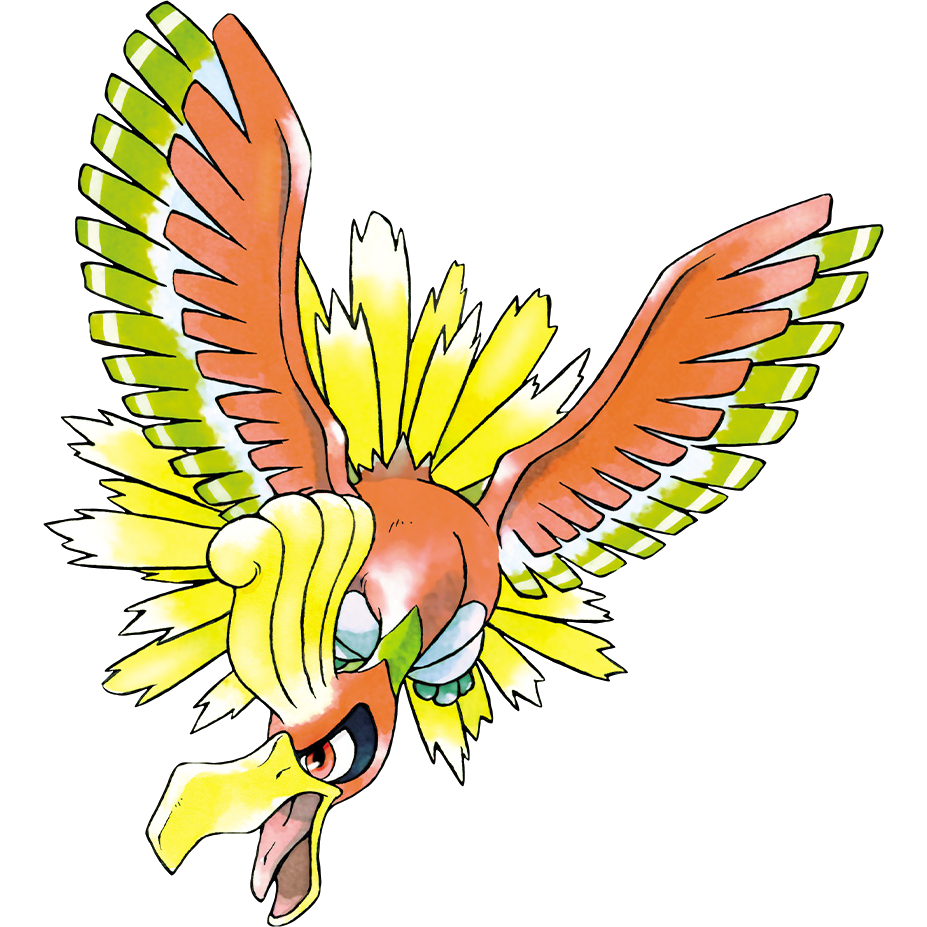
\includegraphics[scale=0.4]{../Graphics/1. Logo.png}}
\begin{document}
\singlespacing
\maketitle
\tableofcontents
\addtocontents{toc}{\vspace{-1cm}}

%----------acknowledgements----------%
\section*{Acknowledgements}
Lembox, sizzleskeleton, MrTyton

\newpage
\chapter{Beginning}
\vspace{0.5mm}

\begin{menu}[hbox]{Before the Run}
	\varwb
	\begin{optionMenu}
		\item \menuHl{(1)} \textbf{Text Speed:} \textSpeed{} \menuHlTwo{\textbf{(\pointLeft)}}
		\item \menuHl{(2)} \textbf{Battle Scene:} \battleScene{} \menuHlTwo{\textbf{(\pointLeft)}}
		\item \menuHl{(3)} \textbf{Battle Style:} \battleStyle{} \menuHlTwo{\textbf{(\pointLeft)}}
		\item \menuHl{(4)} \textbf{Audio:} \audio{} \menuHlTwo{\textbf{(\pointLeft)}}
		\item \menuHl{(6)} \textbf{Menu Account:} \menuAccount{} \menuHlTwo{\textbf{(\pointLeft)}}
	\end{optionMenu}
	\varwe
\end{menu}

\begin{misc}[hbox]{HM Pokemon}
	\varwb
	\begin{notes}
		\item \textbf{Totodile:} Surf and Strength
		\item \textbf{Poliwag or Poliwhirl:} Whirlpool and Waterfall
		\item \textbf{Sentret, Bellsprout, Sandshrew, Oddish, or Paras:} Cut
	\end{notes}
	\varwe
\end{misc}

\vspace{3.5mm}
\chapter{New Bark Town}
\vspace{0.5mm}

\begin{paracol}{2}
\begin{story}{Introduction}
	\varwb
	\begin{notes}
		\item \textbf{Time:} \storyHl{(\pointUp)} \timeStart{}
		\item \textbf{Name:} \textbf{\jp{ア}}
		\item \textbf{Day:} Sunday
		\item \textbf{DST:} Yes
		\item \textbf{Okay:} Yes
		\item \textbf{Phone:} Yes
		\item \textbf{Totodile:} \textbf{\jp{ア}}
	\end{notes}
	\varwe
\end{story}

\begin{menu}{After Getting Totodile}
	\varwb
	\begin{pokeMenuNoPokedex}
		\item \textbf{Totodile} \pointRight{} Stats \menuHlTwo{(1)}
		\item \textbf{Totodile} \pointRight{} Item \menuHlTwo{(2\pointUp)} \pointRight{} \textbf{Take} \menuHlTwo{(2)}
	\end{pokeMenuNoPokedex}
	\varwe
\end{menu}

\switchcolumn
\begin{misc}{Totodile's Stats}
	\varwb
	\begin{notes}
		\item Reset if Totodile is female (low attack DV)
		\item \textul{Target stats:}
		\begin{itemize}
			\item \textbf{\atkDV{12} / x / \spcDV{10 / 10} / 10}
			\item \textbf{\atkDV{12} / x / \spcDV{10 / 11} / 9}
		\end{itemize}
		\item \textul{Ideal stats:}
		\begin{itemize}
			\item \textbf{\atkDV{12} / x / \spcDV{10 / 11} / 10}
			\item \textbf{\atkDV{13} / x / \spcDV{10 / 10} / 10}
		\end{itemize}
		\item \textul{Runnable stats:}
		\begin{itemize}
			\item \textbf{\atkDV{12} / x / \spcDV{10 / 10} / 9}
			\item \textbf{\atkDV{13} / x / \spcDV{9 / 9} / 9}
		\end{itemize}
	\end{notes}
	\varwe
\end{misc}

\begin{encounter}{If Totodile Has 11 DEF (second stat)}
	\varwb
	\begin{notes}
		\item \encounterHl{(1)} \scratch{} encounters to hit L6
	\end{notes}
	\varwe
\end{encounter}

\switchcolumn
\begin{enumerate}
	\item Make your way to Mr. Pokemon and grab the hidden \pickup{Potion}
	\item Grab the \pickup{Berry} on the left side of the house on the way back to Professor Elm
\end{enumerate}

\switchcolumn
\begin{items}{Hidden Potion}
	\varwb
	\insertScreenshot{../Graphics/2. Hidden Potion.png}
	\varwe
\end{items}

\switchcolumn
\begin{boss}{Rival \#1}
	\varwb
	\begin{fightSection}{Chikorita}
		\item \bossHl{(2)} \leer{}
		\item \bossHl{(1)} \scratch{}
	\end{fightSection}
	\varwe
\end{boss}

\switchcolumn
\begin{encounter}{Catch a Sentret For Cut on Route 29 If You Encounter One}
	\varwb
	\begin{notes}
		\item \encounterHl{(1)} \scratch{}
		\item \pokeBall{} \encounterHlTwo{(\pointRight)}
	\end{notes}
	\varwe
\end{encounter}

\switchcolumn
\begin{enumerate}[resume]
	\item Name your rival \textbf{\jp{ア}} then \dialog{talk to Professor Elm}
	\item \dialog{Skip the catching tutorial on the way out of New Bark Town}
	\item Grab the \pickup{Berry} on the second pass
	\item Avoid the first trainer through the grass
\end{enumerate}

\begin{trainer}{Youngster Mikey}
	\varwb
	\begin{fightSection}{Pidgey}
		\item \trainerSwap{\textbf{(1)} \scratch{} \switch{} \textbf{(3)} \rage{} \textit{(if L7)}}
		\item \trainerHl{(3)} \scratch{} \trainerHlTwo{2x}
		\begin{notes}
			\small{\item \trainerHl{(1)} \rage{} \trainerHlTwo{2x} \textit{(if L7)}}
		\end{notes}
	\end{fightSection}
	\begin{fightSection}{Rattata}
		\item \trainerHl{(3)} \scratch{} \trainerHlTwo{3x}
		\begin{notes}
			\small{\item \trainerHl{(1)} \rage{} \trainerHlTwo{2x} \textit{(if L7)}}
		\end{notes}
	\end{fightSection}
	\varwe
\end{trainer}

\begin{enumerate}[resume]
	\item \emphasis{Avoid spinner: Bugcatcher Don}
\end{enumerate}

\switchcolumn*
\begin{trainer}{If Caught by Bugcatcher Don}
	\varwb
	\begin{fightSection}{Caterpie/Caterpie}
		\item \trainerSwap{\textbf{(1)} \scratch{} \switch{} \textbf{(3)} \rage{} \textit{(if not done already)}}
		\item \trainerHl{(1)} \rage
	\end{fightSection}
	\varwe
\end{trainer}

\switchcolumn
\begin{menu}{Buffering Bugcatcher Don}
	\varwb
	\begin{packMenu}
		\item \textbf{\berry{}} \pointRight{} Give \menuHlTwo{(2)}
		\begin{notes}
			\small{\item Use \menuHlTwo{(1)} \textit{(if $\leq$19 HP or bad DEF)}}
		\end{notes}
	\end{packMenu}
	\begin{gearMenu}
		\item \textbf{Phone \menuHlTwo{(2)}} \pointRight{} Mom \menuHlTwo{(1)} \pointRight{} \textbf{Call \menuHlTwo{(1)}}
		\begin{notes}
			\item Stop saving money \menuHlTwo{(2)}
		\end{notes}
	\end{gearMenu}
	\varwe
\end{menu}

\begin{enumerate}[resume]
	\item Run from Bellsprouts to avoid unnecessary damage
	\item Grab the \pickup{Bitter Berry}
\end{enumerate}

\end{paracol}
\vspace{3.5mm}
\chapter{Violet Town}
\vspace{0.5mm}

\begin{paracol}{2}
\begin{enumerate}
	\item Head to Falkner's Gym (northwest)
\end{enumerate}

\switchcolumn
\begin{menu}{Conditional Menu Before Abe}
	\varwb
	\begin{packMenu}
		\item \berry{} \textbf{or} \potion{}
		\item \textbf{\berry{}} \pointRight{} Give \menuHlTwo{(2)}
	\end{packMenu}
	\varwe
\end{menu}

\begin{menu}{Conditional Heal Between Trainers}
	\varwb
	\begin{packMenu}
		\item \emphasis{Heal if $\leq$9 HP}
		\item \berry{} \textbf{or} \potion{}
		\item \textbf{\bitterBerry{}} \pointRight{} Give \menuHlTwo{(1)}
	\end{packMenu}
	\varwe
\end{menu}

\switchcolumn
\begin{trainer}{Bird Keeper Abe}
	\varwb
	\begin{fightSection}{Spearow}
		\item \trainerSwap{\textbf{(1)} \scratch{} \switch{} \textbf{(3)} \rage{} \textit{(if not done already)}}
		\item \trainerHl{(1)} \rage{} \trainerHlTwo{3x}
		\begin{notes}
			\small{\item \trainerHl{(3)} \scratch{} \textit{(if necessary)}}
		\end{notes}
	\end{fightSection}
	\varwe
\end{trainer}

\switchcolumn
\begin{menu}{Conditional Healing Before Falkner}
	\varwb
	\begin{packMenu}
		\item \emphasis{Heal if $\leq$17 HP @9 \textbf{or} $\leq$19 HP @10}
		\item \berry{} \textbf{or} \potion{} 
		\item \textbf{\bitterBerry{}} \pointRight{} Give \menuHlTwo{(1)}
		\begin{notes}
			\small{\item \textit{If not done already}}
		\end{notes}
	\end{packMenu}
	\varwe
\end{menu}

\switchcolumn
\begin{trainer}{Bird Keeper Rod}
	\varwb
	\begin{fightSection}{Pidgey/Pidgey}
		\item \trainerHl{(1)} \rage{}
	\end{fightSection}
	\varwe
\end{trainer}

\begin{boss}{Falkner}
	\varwb
	\begin{fightSection}{Pidgey/Pidgeotto}
		\item \bossHl{(1)} \rage{}
	\end{fightSection}
	\varwe
\end{boss}

\begin{enumerate}[resume]
	\item Head to the Pokemon Center (southeast)
	\item \emphasis{Heal} and get the \dialog{Egg from the guy near the counter (hold A)}
	\item Exit Violet Town by heading north \pointRight{} west \pointRight{} south
	\item Grab the \pickup{PRZCureBerry} and continue south
\end{enumerate}

\switchcolumn
\begin{encounter}{Catch a Bellsprout on Route 32 For Cut If Needed}
	\varwb
	\begin{notes}
		\item \encounterHl{(3)} \scratch
		\item \pokeBall{} \encounterHlTwo{(\pointRight)}
	\end{notes}
	\varwe
\end{encounter}

\switchcolumn
\begin{trainer}{Youngster Albert}
	\varwb
	\begin{fightSection}{Rattata/Zubat}
		\item \trainerHl{(3)} \scratch
		\begin{notes}
			\small{\item \trainerHl{(1)} \rage{} \textit{(if 15 DV ATK)}}
		\end{notes}
	\end{fightSection}
	\varwe
\end{trainer}

\begin{enumerate}[resume]
	\item Grab the hidden \pickup{Super Potion}
\end{enumerate}

\switchcolumn
\begin{items}{Hidden Super Potion}
	\varwb
	\insertScreenshot{../Graphics/3. Hidden Super Potion.png}
	\varwe
\end{items}

\switchcolumn
\begin{trainer}{Fisher Ralph (Facing Upwards)}
	\varwb
	\begin{fightSection}{Goldeen}
		\item \trainerHl{(2)} \leer
		\item \trainerHl{(3)} \scratch
		\begin{notes}
			\small{\item Skip Leer \textit{(if 12-15 DV ATK)}}
		\end{notes}
	\end{fightSection}
	\varwe
\end{trainer}

\begin{enumerate}[resume]
	\item \emphasis{Avoid rotator}
	\item \emphasis{Stick to the left side before the cave}
\end{enumerate}

\begin{encounter}{Defeat Encounters That Can Be One-Shot By Water Gun}
	\varwb
	\begin{fightSection}{Rattata/Geodude/Onix}
		\item \encounterHl{(4)} \waterGun
	\end{fightSection}
	\varwe
\end{encounter}

\switchcolumn
\begin{encounter}{Catch a Sandshrew on Route 33 For Cut If Needed}
	\varwb
	\begin{notes}
		\item \encounterHl{(3)} \scratch{} \encounterHlTwo{2x}
		\item \pokeBall{} \encounterHlTwo{(\pointRight)}
	\end{notes}
	\varwe
\end{encounter}

\switchcolumnTwice[*]
\begin{trainer}{Hiker Daniel}
	\varwb
	\begin{fightSection}{Onix}
		\item \trainerHl{(4)} \waterGun
	\end{fightSection}
	\varwe
\end{trainer}

\switchcolumn
\begin{enumerate}[resume]
	\item \emphasis{Avoid spinner: Hiker Daniel (pass aggressively)}
\end{enumerate}

\begin{trainer}{Hiker Russel}
	\varwb
	\begin{fightSection}{Geodude/Geodude/Geodude}
		\item \trainerHl{(4)} \waterGun
	\end{fightSection}
	\varwe
\end{trainer}

\switchcolumnTwice[*]
\begin{enumerate}[resume]
	\item \emphasis{Avoid spinner: Firebreather Bill}
	\item Head left past Bill \pointRight{} down \pointRight{} right (past water) \pointRight{} down
\end{enumerate}

\switchcolumn
\begin{trainer}{Firebreather Bill}
	\varwb
	\begin{fightSection}{Koffing/Koffing}
		\item \trainerHl{(4)} \waterGun
	\end{fightSection}
	\varwe
\end{trainer}

\switchcolumn
\begin{trainer}{Firebreather Ray}
	\varwb
	\begin{fightSection}{Vulpix}
		\item \trainerHl{(4)} \waterGun
		\item \trainerHl{(3)} \scratch
	\end{fightSection}
	\varwe
\end{trainer}

\switchcolumnTwice[*]
\begin{enumerate}[resume]
	\item \emphasis{Avoid spinner: Hiker Anthony}
\end{enumerate}

\begin{menu}{Buffering Hiker Anthony}
	\varwb
	\begin{packMenu}
		\item \textbf{\potion{}} \textit{(if it nearly heals to full)}
		\begin{notes}
			\small{\item \textbf{\superPotion{}} \textit{(otherwise)}}
		\end{notes}
		\item \menuHlTwo{If BRN heal later}
	\end{packMenu}
	\varwe
\end{menu}

\switchcolumn
\alignBoxes
\begin{trainer}{Hiker Anthony}
	\varwb
	\begin{fightSection}{Geodude/Machop}
		\item \trainerHl{(4)} \waterGun
	\end{fightSection}
	\varwe
\end{trainer}

\end{paracol}
\vspace{3.5mm}
\chapter{Azalea Town}
\vspace{0.5mm}

\begin{paracol}{2}
\begin{enumerate}
	\item Head to Kurt (west past the Pokemon Center, then north) and \dialog{speak to him}
	\item Head to the Mart (east past the Pokemon Center, then north)
\end{enumerate}

\begin{shop}{Azalea Town Mart}
	\varwb
	\begin{buy}
		\item \shopHl{(3\pointDown)} \superPotion{} \shopHlTwo{5x}
		\item \shopHl{(2\pointDown)} \repel{} \shopHlTwo{4x}
		\item \shopHl{(\pointDown)} \antidote{} \shopHlTwo{2x}
		\item \shopHl{(\pointDown)} \paralyzeHeal{} \shopHlTwo{1x}
	\end{buy}
	\varwe
\end{shop}

\begin{enumerate}[resume]
	\item Grab the \pickup{Full Heal} from the middle rock behind the Well entrance, then enter
\end{enumerate}

\switchcolumn*
\begin{menu}{Conditional Menu Before Rocket Grunt \#1}
	\varwb
	\begin{packMenu}
		\item \potion{}
		\begin{notes}
			\small{\item \textbf{\fullHeal{}} \textit{(if not done already)}}
		\end{notes}
	\end{packMenu}
	\varwe
\end{menu}

\switchcolumn
\begin{trainer}{Rocket Grunt \#1}
	\varwb
	\begin{fightSection}{Rattata/Rattata}
		\item \trainerHl{(4)} \waterGun
	\end{fightSection}
	\varwe
\end{trainer}

\switchcolumn
\begin{menu}{Conditional Heal Before Rocket Grunts \#2-4}
	\varwb
	\begin{packMenu}
		\item \textbf{\potion{}} \textit{(if necessary)}
	\end{packMenu}
	\varwe
\end{menu}

\switchcolumn
\begin{trainer}{Rocket Grunt \#2}
	\varwb
	\begin{fightSection}{Zubat/Ekans}
		\item \trainerHl{(4)} \waterGun
		\begin{notes}
			\small{\item \trainerHl{(3)} \scratch{} \textit{(if 15 DV ATK)}}
		\end{notes}
	\end{fightSection}
	\varwe
\end{trainer}

\begin{trainer}{Rocket Grunt \#3}
	\varwb
	\begin{fightSection}{Rattata/Zubat/Zubat}
		\item \trainerHl{(1)} \rage
		\begin{notes}
			\small{\item \trainerHl{(4)} \waterGun{} \textit{(if you don't get hit by Rattata and Zubat)}}
		\end{notes}
	\end{fightSection}
	\varwe
\end{trainer}

\begin{trainer}{Rocket Grunt \#4}
	\varwb
	\begin{fightSection}{Koffing}
		\item \trainerHl{(4)} \waterGun{}
	\end{fightSection}
	\varwe
\end{trainer}

\begin{enumerate}[resume]
	\item Head south to Bugsy's Gym
\end{enumerate}

\switchcolumn*
\begin{trainer}{Twins Amy \& May}
	\varwb
	\begin{notes}
		\item \trainerHlTwo{Otherwise}
	\end{notes}
	\begin{fightSection}{Ledyba}
		\item \trainerHl{(3)} \scratch{} \trainerHlTwo{2x}
	\end{fightSection}
	\varwe
\end{trainer}

\switchcolumn
\begin{trainer}{Twins Amy \& May}
	\varwb
	\begin{notes}
		\item \trainerHlTwo{If no Bitter Berry}
	\end{notes}
	\begin{fightSection}{Spinarak}
		\item \trainerHl{(4)} \waterGun{} \trainerHlTwo{2x}
		\begin{notes}
			\small{\item \trainerHl{(3)} \scratch{} \trainerHlTwo{2x} \textit{(if optional EXP or 15 DV ATK)}}
		\end{notes}
	\end{fightSection}
	\varwe
\end{trainer}

\vspace{-0.4pc}
\begin{enumerate}[resume]
	\item \emphasis{Do not heal if \poison[ed]}
\end{enumerate}

\begin{trainer}{Bug Catcher Josh (Left Trainer)}
	\varwb
	\begin{fightSection}{Paras}
		\item \trainerHl{(2)} \leer
		\item \trainerHl{(3)} \scratch{} \trainerHlTwo{2-3x}
		\begin{notes}
			\small{\item \trainerHl{(1)} \rage{} \trainerHlTwo{3x} \textit{(if poisoned)}}
		\end{notes}
	\end{fightSection}
	\varwe
\end{trainer}

\switchcolumn*
\vspace{0.05pc}
\begin{misc}{Croconaw Evolution (L18)}
	\varwb
	\begin{notes}
		\item \emphasis{Make sure to not be holding B when Totodile evolves}
	\end{notes}
	\varwe
\end{misc}

\begin{trainer}{Bug Catcher Benny}
	\varwb
	\begin{fightSection}{Weedle}
		\item \trainerHl{(4)} \waterGun
	\end{fightSection}
	\begin{fightSection}{Kakuna}
		\item \trainerHl{(4)} \waterGun
		\item \trainerHl{(1)} \rage
	\end{fightSection}
	\begin{fightSection}{Beedrill}
		\item \trainerHl{(1)} \rage
	\end{fightSection}
	\varwe
\end{trainer}

\switchcolumn
\vspace{-0.4pc}
\begin{enumerate}[resume]
	\item \emphasis{Avoid spinner: Bug Catcher Benny}
\end{enumerate}
\vspace{-0.25pc}

\begin{menu}{Buffering Bug Catcher Benny}
	\varwb
	\begin{packMenu}
		\item \textbf{\przCureBerry{}} \pointRight{} Give \menuHlTwo{(2)}
		\item \potion{} \textbf{or} \superPotion{}
		\small{\item \textbf{\antidote{}} \emphasis{\poison{}} \textit{(if necessary)}}
		\small{\item \textbf{\paralyzeHeal{}} \emphasis{\paralyze{}} \textit{(if necessary)}}
	\end{packMenu}
	\varwe
\end{menu}

\begin{boss}{Bugsy}
	\varwb
	\begin{fightSection}{Metapod/Kakuna/Scyther}
		\item \bossHl{(1)} \rage{}
		\begin{notes}
			\small{\item \bossHl{(4)} \waterGun{} Metapod \emphasis{once} \textit{(if Croconaw already)}}
		\end{notes}
	\end{fightSection}
	\varwe
\end{boss}

\begin{menu}{Before Rival \#2}
	\varwb
	\begin{packMenu}
		\item \superPotion
		\item \repel{} \textit{(unless you need an Oddish/Paras)}
		\item \menuHlTwo{(\pointLeft{})} \tm{49} \furyCutter{} \switch{} \rage{} \menuHlTwo{(1)}
	\end{packMenu}
	\varwe
\end{menu}

\begin{enumerate}[resume]
	\item Attempt to exit Azalea Town to the west
\end{enumerate}

\begin{boss}{Rival \#2}
	\varwb
	\begin{fightSection}{Gastly}
		\item \bossHl{(4)} \waterGun{} \bossHlTwo{2x}
	\end{fightSection}
	\begin{fightSection}{Bayleef}
		\item \bossHl{(1)} \furyCutter{} \bossHlTwo{3x}
	\end{fightSection}
	\begin{fightSection}{Zubat}
		\item \bossHl{(4)} \waterGun{} \bossHlTwo{2-3x}
	\end{fightSection}
	\varwe
\end{boss}

\begin{enumerate}[resume]
	\item Use Repels unless you need an Oddish/Paras
	\item Continue following the Farfetch'd and get \dialog{HM01 (Cut) from the left guy at the end}
\end{enumerate}

\switchcolumn
\newpage
\begin{encounter}{Last Chance to Get a Pokemon for Cut}
	\varwb
	\begin{fightSection}{Oddish/Paras}
		\item \encounterHl{(4)} \waterGun
		\item \pokeBall{} \encounterHlTwo{(\pointRight)}
	\end{fightSection}
	\varwe
\end{encounter}

\switchcolumn
\begin{menu}{When Repel Runs Out}
	\varwb
	\begin{packMenu}
		\item \repel
		\item \menuHlTwo{(\pointLeft{})} \hm{1} \cut{}
	\end{packMenu}
	\varwe
\end{menu}

\switchcolumnTwice[*]
\begin{enumerate}[resume]
	\item Use Cut on the tree and continue northwest
	\item Continue following the path east and south and get \dialog{TM02 (Headbutt) from the guy}
	\item Jump off the ledge and take the north path
	\item Left of the sign \pointRight{} \emphasis{left edge of the grass to avoid the girl on the left}
	\item Hug the left wall \pointRight{} \emphasis{move one additional tile left when you are able}
\end{enumerate}

\switchcolumn
\begin{menu}{When Repel Runs Out}
	\varwb
	\begin{packMenu}
		\item \menuHlTwo{(\pointLeft{})} \tm{2} \headbutt{} \switch{} \leer{} \menuHlTwo{(2)}
		\begin{notes}
			\item \emphasis{Do not teach Headbutt to your Cut Pokemon}
		\end{notes}
		\item \repel
	\end{packMenu}
	\varwe
\end{menu}

\end{paracol}
\vspace{3.5mm}
\chapter{Goldenrod City}
\vspace{0.5mm}

\begin{paracol}{2}
\begin{enumerate}
	\item Head north until you are above the big building
	\item Head east and south until you reach the Bike Shop
	\item \dialog{Speak to the clerk (hold A) to get the Bike}
\end{enumerate}

\begin{menu}{After Getting the Bike}
	\varwb
	\begin{packMenu}
		\small{\item \superPotion{} \textit{(if necessary)}}
		\item \menuHlTwo{(2\pointLeft)} Register the \bike{} \menuHlTwo{(2)}
		\item Use the \bike{} \menuHlTwo{(1)}
	\end{packMenu}
	\varwe
\end{menu}

\begin{enumerate}[resume]
	\item Head to Whitney's Gym (back up the path and north)
	\item Take the left path and \emphasis{keep to the right to avoid a trainer}
\end{enumerate}

\begin{trainer}{Lass Carrie}
	\varwb
	\begin{fightSection}{Snubbull}
		\item \trainerHl{(2)} \headbutt{} \trainerHlTwo{3x}
		\begin{notes}
			\small{\item \trainerHl{(4)} \waterGun{} \textit{(if Charmed)}}
		\end{notes}
	\end{fightSection}
	\varwe
\end{trainer}

\begin{menu}{Before Whitney}
	\varwb
	\begin{packMenu}
		\item \superPotion
	\end{packMenu}
	\varwe
\end{menu}

\switchcolumn
\vspace{12.05cm}
\begin{misc}{When You Hit L21}
	\varwb
	\begin{notes}
		\item \emphasis{Make sure to not be holding B so you can learn Bite}
	\end{notes}
	\varwe
\end{misc}

\switchcolumn
\begin{boss}{Whitney}
	\varwb
	\begin{fightSection}{Clefairy}
		\item \bossHl{(1)} \furyCutter{}
		\item[]
		\item \bossNote{Learn \bite{} \switch{} \textbf{(3)} \scratch{} \textit{(if still fighting)}}
		\item[]
	\end{fightSection}
	\begin{fightSection}{Miltank}
		\item \textbf{Miltank defeats you with \emphasis{21 HP} (0 DV DEF) to \emphasis{19 HP} (15 DV DEF)}
		\item \bossHl{(1)} \furyCutter{} \bossHlTwo{(ideally 1x)}
		\begin{notes}
			\small{\item \bossHl{(2)} \headbutt{} \textit{(if Miltank has low HP and uses} \rollout \textit{)}}
			\small{\item \bossHl{(1)} \furyCutter{} \textit{(otherwise)}}
		\end{notes}
		\item[]
		\item \bossNote{Learn \bite{} \switch{} \textbf{(1)} \furyCutter{}}
	\end{fightSection}
	\varwe
\end{boss}

\begin{enumerate}[resume]
	\item \dialog{Attempt to leave then talk to Whitney again}
	\item \dialog{Talk to the woman in the top house on the right to get the Squirt Bottle}
	\item \dialog{Get Kenya from the guy on the left in the gate to the north (hold A)}
	\item Head to the underground (south and then west at the first path into the small house) and fight the top two trainers
\end{enumerate}

\begin{trainer}{Pokemaniac Donald}
	\varwb
	\begin{notes}
		\small{\item \trainerSwap{\textbf{(3)} \bite{} \switch{} \textbf{(1)} \furyCutter}}
		\begin{notes}
			\small{\item \trainerHlThreeNoBold{\textit{If you learned Bite early}}}
		\end{notes}
	\end{notes}
	\begin{fightSection}{Slowpoke/Slowpoke}
		\item \trainerHl{(1)} \bite{} \trainerHlTwo{2x}
		\begin{notes}
			\small{\item \trainerHl{(2)} \headbutt{} \trainerHlTwo{2x} \textit{(if 13+ DV ATK)}}
		\end{notes}
	\end{fightSection}
	\varwe
\end{trainer}

\resume
\begin{enumerate}[resume]
	\item \dialog{Talk to the second trainer to fight him}
\end{enumerate}

\begin{trainer}{Super Nerd Teru}
	\varwb
	\begin{fightSection}{Magnemite/Magnemite/Magnemite}
		\item \trainerHl{(4)} \waterGun{} \trainerHlTwo{3x}
	\end{fightSection}
	\begin{fightSection}{Voltorb}
		\item \trainerHl{(2)} \headbutt
	\end{fightSection}
	\varwe
\end{trainer}

\switchcolumn*
\alignBoxes
\begin{items}{Hidden Super Potion}
	\varwb
	\insertScreenshot{../Graphics/4. Hidden Super Potion.png}
	\varwe
\end{items}

\switchcolumn
\begin{enumerate}[resume]
	\item Grab the \pickup{Coin Case} and the hidden \pickup{Super Potion}
	\item Head to the Radio Tower and talk to the middle NPC to get the \pickup{Master Ball}
\end{enumerate}

\begin{story}{Radio Tower PC}
	\varwb
	\begin{pokeMenuStory}
		\item \textbf{Bill's PC} \storyHlTwo{(1)} \pointRight{} Deposit \storyHlTwo{(2)} \pointRight{} Croconaw and Egg
		\item \textbf{Back one screen} \storyHlTwo{(B)} \pointRight{} Withdraw \storyHlTwo{(1)} \pointRight{} Croconaw
	\end{pokeMenuStory}
	\varwe
\end{story}

\begin{enumerate}[resume]
	\item Head to the Game Corner (south and west across from the large building)
\end{enumerate}

\begin{shop}{Game Corner}
	\varwb
	\begin{shopSection}{Far left clerk}
		\item \shopHl{(1)} 50 Coins \shopHlTwo{4x}
	\end{shopSection}
	\begin{shopSection}{Far right clerk}
		\item \shopHl{(1)} \abra
	\end{shopSection}
	\varwe
\end{shop}

\begin{enumerate}[resume]
	\item Head to the Mart (large building on the right)
\end{enumerate}

\begin{shop}{Goldenrod City Mart}
	\varwb
	\begin{notes}
		\item \textbf{Floor 3}
	\end{notes}
	\begin{sell}
		\item  \tm{31} \mudSlap
		\item \tm{45} \attract
	\end{sell}
	\begin{buy}
		\item \shopHl{(A)} \xSpeed
		\item \shopHl{(\pointDown)} \xSpecial
		\item \shopHl{(2\pointDown)} \xAttack{} \shopHlTwo{2x}
	\end{buy}
	\begin{notes}
		\item \textbf{Floor 2 (bottom clerk)}
	\end{notes}
	\begin{buy}
		\item \shopHl{(2\pointDown)} \escapeRope{} \shopHlTwo{5x}
		\item \shopHl{(3\pointDown)} \fullHeal{} \shopHlTwo{3x}
	\end{buy}
	\varwe
\end{shop}

\newpage
\begin{menu}{After Exiting the Mart}
	\varwb
	\begin{pokeMenu}
		\item \textbf{\abra{}} \pointRight{} \teleport{} \menuHlTwo{(1)}
	\end{pokeMenu}
	\varwe
\end{menu}

\vspace{-0.4pc}
\begin{enumerate}[resume]
	\item Head northwest from Violet Town towards Sudowoodo
\end{enumerate}

\begin{menu}{After Arriving at Sudowoodo}
	\varwb
	\begin{pokeMenu}
		\item Swap \menuHl{(3)} Cut Pokemon \switch{} Croconaw
	\end{pokeMenu}
	\begin{packMenu}
		\item \menuHlTwo{(2\pointLeft)} \squirtBottle
	\end{packMenu}
	\varwe
\end{menu}

\vspace{-0.4pc}
\begin{enumerate}[resume]
	\item \emphasis{Head north and stick just left of the sign to avoid a trainer}
\end{enumerate}

\begin{trainer}{Psychic Greg}
	\varwb
	\begin{fightSection}{Drowzee}
		\item \trainerHl{(2)} \headbutt
		\item \trainerHl{(1)} \bite
	\end{fightSection}
	\varwe
\end{trainer}

\end{paracol}
\vspace{3.5mm}
\chapter{Ecruteak City}
\vspace{0.5mm}

\begin{paracol}{2}
\begin{enumerate}
	\item Grab the hidden \pickup{Hyper Potion} if low on healing items
	\item Head to the second house on the right (an old man is standing beside the sign)
\end{enumerate}

\switchcolumn
\begin{items}{Hidden Hyper Potion}
	\varwb
	\insertScreenshot{../Graphics/5. Hidden Hyper Potion.png}
	\varwe
\end{items}

\switchcolumn
\begin{trainer}{Kimono Girls}
	\varwb
	\begin{notes}
		\item \trainerHlThree{9-12 DV SPD} \pointRight{} right to left
		\item \trainerHlThree{Otherwise} \pointRight{} left to right
	\end{notes}
	\begin{fightSection}{Flareon}
		\item \trainerHl{(2)} \headbutt{} \trainerHlTwo{2x}
	\end{fightSection}
	\begin{fightSection}{Espeon}
		\item \trainerHl{(2)} \headbutt{} \trainerHlTwo{2x}
		\item \trainerHl{(1)} \bite{}
	\end{fightSection}
	\begin{fightSection}{Umbreon}
		\item \trainerHl{(2)} \headbutt{} \trainerHlTwo{3x}
		\item \trainerHl{(4)} \waterGun{}
	\end{fightSection}
	\begin{fightSection}{Vaporeon}
		\item \trainerHl{(2)} \headbutt{} \trainerHlTwo{2x}
		\item \trainerHl{(1)} \bite{}
	\end{fightSection}
	\begin{notes}
		\item \trainerHlTwo{Heal if $<$45 HP}
	\end{notes}
	\begin{fightSection}{Jolteon}
		\item \trainerHl{(2)} \headbutt{}
		\item \trainerHl{(3)} \scratch{}
	\end{fightSection}
	\varwe
\end{trainer}

\switchcolumn
\begin{menu}{Conditional Heal Before Jolteon}
	\varwb
	\begin{packMenu}
		\item \superPotion{} \textit{(if $<$45 HP)}
	\end{packMenu}
	\varwe
\end{menu}

\switchcolumn
\begin{enumerate}[resume]
	\item \dialog{Get HM03 (Surf) from the man with the hat}
\end{enumerate}

\begin{menu}{After Getting Surf}
	\varwb
	\begin{packMenu}
		\small{\item \superPotion{} \textit{(if necessary)}}
		\item \menuHlTwo{(\pointLeft{})} \textbf{H3 \surf{}} \switch{} \scratch{} \menuHlTwo{(3)}
		\item \bike
	\end{packMenu}
	\varwe
\end{menu}

\begin{enumerate}[resume]
	\item Head southwest to Morty's Gym
\end{enumerate}

\switchcolumn
\vspace{4.7cm}
\begin{story}{Morty's Gym Path}
	\varwb
	\insertPath{../Graphics/6. Morty's Gym.png}
	\varwe
\end{story}

\switchcolumn
\begin{trainer}{Sage Ping}
	\varwb
	\begin{fightSection}{Gastly/Gastly/Gastly/Gastly/Gastly}
		\item \trainerSwap{\textbf{(1)} \bite{} \switch{} \textbf{(3)} \surf}
		\item \trainerHl{(1)} \surf{} \trainerHlTwo{5x}
	\end{fightSection}
	\varwe
\end{trainer}

\begin{trainer}{Sage Jeffrey}
	\varwb
	\begin{fightSection}{Haunter}
		\item \trainerHl{(3)} \bite{} \trainerHlTwo{2x}
		\begin{notes}
			\small{\item \trainerHl{(3)} \bite{} + \trainerHl{(4)} \waterGun{} \textit{(if 15 DV SPC)}}
		\end{notes}
	\end{fightSection}
	\varwe
\end{trainer}

\switchcolumn
\begin{menu}{Conditional Heal Before Morty}
	\varwb
	\begin{packMenu}
		\item \superPotion{} \textit{(if necessary)}
	\end{packMenu}
	\varwe
\end{menu}

\begin{misc}{When You Hit L28}
	\varwb
	\begin{notes}
		\item \emphasis{B \pointRight{} A to cancel learning Scary Face}
	\end{notes}
	\varwe
\end{misc}

\switchcolumn
\begin{trainer}{Medium Martha}
	\varwb
	\begin{fightSection}{Gastly}
		\item \trainerHl{(1)} \surf
	\end{fightSection}
	\begin{fightSection}{Haunter}
		\item \trainerHl{(3)} \bite
		\item \trainerHl{(4)} \waterGun
	\end{fightSection}
	\begin{fightSection}{Gastly}
		\item \trainerHl{(1)} \surf
	\end{fightSection}
	\varwe
\end{trainer}

\begin{boss}{Morty}
	\varwb
	\begin{fightSection}{Gastly}
		\item \xSpeed
		\item \xSpecial
		\item \bossSwap{\textbf{(1)} \surf{} \switch{} \textbf{(4)} \waterGun}
		\item \bossHl{(3)} \bite{}
		\begin{notes}
			\small{\item \bossHl{(1)} \waterGun{} \textit{(if Curse)}}
		\end{notes}
	\end{fightSection}
	\begin{fightSection}{Haunter}
		\item \bossHl{(3)} \bite
	\end{fightSection}
	\begin{fightSection}{Gengar}
		\item \bossHl{(3)} \bite
		\item \bossHl{(4)} \surf
	\end{fightSection}
	\begin{fightSection}{Haunter}
		\item \bossHl{(4)} \surf
	\end{fightSection}
	\varwe
\end{boss}

\begin{menu}{Before Route 38}
	\varwb
	\begin{packMenu}
		\small{\item \superPotion{} \textit{(if necessary)}}
		\item \repel 
		\item \bike
	\end{packMenu}
	\varwe
\end{menu}

\begin{enumerate}[resume]
	\item Head west and bike down Route 38
	\item Stay near the bottom and then up the patch of grass \emphasis{(staying on the left side)}
	\item Head south and \emphasis{stick to the left side, jumping off the ledges}
\end{enumerate}

\end{paracol}
\vspace{3.5mm}
\chapter{Olivine City}
\vspace{0.5mm}

\begin{paracol}{2}
\begin{enumerate}
	\item Head south to the Mart
\end{enumerate}

\begin{shop}{Azalea Town Mart}
	\varwb
	\begin{buy}
		\item \shopHl{(\pointDown)} \superPotion{} \shopHlTwo{2-3x}
		\item \shopHl{(6\pointDown)} \superRepel{} \shopHlTwo{11x}
	\end{buy}
	\varwe
\end{shop}

\begin{enumerate}[resume]
	\item Head southeast to the the Lighthouse
\end{enumerate}

\begin{trainer}{Gentleman Alfred}
	\varwb
	\begin{fightSection}{Noctowl}
		\item \trainerHl{(2)} \headbutt
		\item \trainerHl{(4)} \surf
	\end{fightSection}
	\varwe
\end{trainer}

\begin{enumerate}[resume]
	\item \emphasis{Be careful of the trainer on your left}
\end{enumerate}

\begin{trainer}{Gentleman Preston}
	\varwb
	\begin{fightSection}{Growlithe/Growlithe}
		\item \trainerHl{(1)} \waterGun{} \trainerHlTwo{(2x)}
		\begin{notes}
			\small{\item \trainerHl{(2)} \headbutt{} \textit{(if $\geq$12 DV ATK)}}
		\end{notes}
	\end{fightSection}
	\varwe
\end{trainer}

\begin{trainer}{Lass Connie}
	\varwb
	\begin{fightSection}{Marill}
		\item \trainerHl{(2)} \headbutt
		\item \trainerHl{(3)} \bite
	\end{fightSection}
	\varwe
\end{trainer}

\switchcolumn*
\begin{trainer}{Sailor Ernest}
	\varwb
	\begin{fightSection}{Machop/Machop}
		\item \trainerHl{(4)} \surf{} \trainerHlTwo{2x}
	\end{fightSection}
	\begin{fightSection}{Poliwhirl}
		\item \trainerHl{(2)} \headbutt
		\item \trainerHl{(3)} \bite
	\end{fightSection}
	\varwe
\end{trainer}

\switchcolumn
\begin{enumerate}[resume]
	\item Go down the left hole \emphasis{on the left side}
	\item \emphasis{Avoid spinner: Sailor Ernest}
	\item \dialog{Talk to Jasmine} then fall down the northeast hole
	\item Head south to grab the \pickup{Rare Candy}
\end{enumerate}

\switchcolumn
\begin{encounter}{If Not L29: Fight a Tentacool on Route 40}
	\varwb
	\begin{notes}
		\item \encounterHl{(2)} \headbutt
	\end{notes}
	\varwe
\end{encounter}

\begin{story}{Feraligatr Evolution}
	\varwb
	\begin{notes}
		\item \emphasis{Make sure to not be holding B when Croconaw evolves}
	\end{notes}
	\varwe
\end{story}

\switchcolumn
\begin{menu}{After Getting the Rare Candy (If L29)}
	\varwb
	\begin{packMenu}
		\item \superPotion
		\item \toss{\antidote} \menuHlTwo{(3)}
		\item \toss{\paralyzeHeal} \menuHlTwo{(3)}
		\item \superRepel
		\item \rareCandy
		\item Move \textbf{\superRepel{}} to the top
		\item \escapeRope
	\end{packMenu}
	\varwe
\end{menu}

\begin{enumerate}[resume]
	\item Head west to get \dialog{HM04 (Strength) from the right guy in the house west of the Pokemon Center}
	\item Head west and Surf (near the girl)
	\item Head south and \emphasis{then west when you see a spinner at the bottom of the screen}
	\item Continue south and west
	\item \emphasis{Avoid spinner: Swimmer Kaylee}
\end{enumerate}

\switchcolumn*
\begin{trainer}{Swimmer Kaylee}
	\varwb
	\begin{fightSection}{Goldeen/Goldeen}
		\item \trainerHl{(1)} \strength{} \trainerHlTwo{2x}
	\end{fightSection}
	\begin{fightSection}{Seaking}
		\item \trainerHl{(2)} \headbutt
		\item \trainerHl{(3)} \bite
	\end{fightSection}
	\varwe
\end{trainer}

\switchcolumn
\begin{menu}{Buffering Swimmer Kaylee}
	\varwb
	\begin{packMenu}
		\item \menuHlTwo{(\pointLeft{})} \textbf{H4 \strength{}} \switch{} \waterGun{} \menuHlTwo{(1)}
	\end{packMenu}
	\varwe
\end{menu}

\begin{enumerate}[resume]
	\item Continue following the wall until you reach land
	\item Head south to Cianwood City
\end{enumerate}

\end{paracol}
\vspace{3.5mm}
\chapter{Cianwood City}
\vspace{0.5mm}

\begin{paracol}{2}
\begin{enumerate}
	\item Head south to Chuck's Gym
\end{enumerate}

\begin{trainer}{Blackbelt Yoshi}
	\varwb
	\begin{fightSection}{Hitmonlee}
		\item \trainerHl{(2)} \headbutt
		\item \trainerHl{(1)} \strength
	\end{fightSection}
	\varwe
\end{trainer}

\begin{trainer}{Blackbelt Lao}
	\varwb
	\begin{fightSection}{Hitmonchan}
		\item \trainerHl{(2)} \headbutt
		\item \trainerHl{(1)} \strength
	\end{fightSection}
	\varwe
\end{trainer}

\begin{trainer}{Blackbelt Nob}
	\varwb
	\begin{fightSection}{Machop}
		\item \trainerHl{(4)} \surf
	\end{fightSection}
	\begin{fightSection}{Machoke}
		\item \trainerHl{(1)} \strength{} \trainerHlTwo{2x}
	\end{fightSection}
	\varwe
\end{trainer}

\begin{trainer}{Blackbelt Lung}
	\varwb
	\begin{fightSection}{Mankey/Mankey/Primeape}
		\item \trainerHl{(1)} \strength{} \trainerHlTwo{4x}
	\end{fightSection}
	\varwe
\end{trainer}

\begin{boss}{Chuck}
	\varwb
	\begin{notes}
		\item \bossHlThree{$\leq$13 DV ATK}
	\end{notes}
	\begin{fightSection}{Primeape}
		\item \xAttack{} \bossHlTwo{2x}
		\item \bossHl{(1)} \strength
	\end{fightSection}
	\begin{fightSection}{Poliwrath}
		\item \bossHl{(2)} \headbutt
		\item \bossHl{(1)} \strength
	\end{fightSection}
	\begin{notes}
		\item \bossHlThree{$\geq$14 DV ATK}
	\end{notes}
	\begin{fightSection}{Primeape}
		\item \xAttack
		\item \bossHl{(1)} \strength
	\end{fightSection}
	\begin{fightSection}{Poliwrath}
		\item \bossHl{(1)} \strength{} \bossHlTwo{2x}
	\end{fightSection}
	\varwe
\end{boss}

\switchcolumn*
\vspace{-2cm}
\begin{story}{Fly to Ecruteak City}
	\varwb
	\insertMap{../Graphics/7. Ecruteak City.png}
	\varwe
\end{story}

\switchcolumn
\begin{enumerate}[resume]
	\item \dialog{Get HM02 (Fly) from Chuck's wife outside the Gym}
	\item Head southeast to the house to \dialog{get the Secret Potion from the man}
\end{enumerate}

\begin{menu}{After Getting the Secret Potion}
	\varwb
	\begin{packMenu}
		\item \superRepel
		\item \menuHlTwo{(\pointLeft{})} H2 \fly{}
	\end{packMenu}
	\begin{pokeMenu}
		\item \menuHlTwo{(1)} \fly{} to Ecruteak City \menuHlTwo{(3\pointDown)}
	\end{pokeMenu}
	\varwe
\end{menu}

\begin{enumerate}[resume]
	\item Head east to Route 42 and Surf east
	\item After arriving, head east and Surf again
	\item \emphasis{Move into the grass to avoid the trainer}
	\item \emphasis{Avoid spinner: Hiker Benjamin}
\end{enumerate}

\switchcolumn*
\vspace{-1cm}
\begin{trainer}{Hiker Benjamin}
	\varwb
	\begin{fightSection}{Diglett/Geodude/Dugtrio}
		\item \trainerHl{(3)} \bite{} \trainerHlTwo{3x}
	\end{fightSection}
	\varwe
\end{trainer}

\end{paracol}
\vspace{3.5mm}
\newpage
\chapter{Mahogany Town}
\vspace{0.5mm}

\begin{paracol}{2}
\begin{enumerate}
	\item Head north from Mahogany town (through the building)
	\item Bike north \emphasis{along the left side of the grass}
	\item Surf after the trainer and \emphasis{go to the right wall before heading north}
	\item Bike north to Lake of Rage
\end{enumerate}

\switchcolumn*
\begin{story}{Fly to Mahogany Town}
	\varwb
	\insertMap{../Graphics/8. Mahogany Town.png}
	\varwe
\end{story}

\switchcolumn
\begin{encounter}{Shiny Gyarados}
	\varwb
	\begin{notes}
		\item \masterBall
	\end{notes}
	\varwe
\end{encounter}

\begin{enumerate}[resume]
	\item \dialog{Talk to Lance before leaving (hold A)}
\end{enumerate}

\begin{menu}{After Talking to Lance}
	\varwb
	\begin{pokeMenu}
		\item \menuHlTwo{(1)} \fly{} to Mahogany Town \menuHlTwo{(2\pointDown)}
	\end{pokeMenu}
	\varwe
\end{menu}

\begin{enumerate}[resume]
	\item Head north to the house and enter Team Rocket Hideout
\end{enumerate}

\begin{trainer}{Rocket Grunt \#1}
	\varwb
	\begin{fightSection}{Drowzee/Zubat}
		\item \trainerHl{(1)} \strength{} \trainerHlTwo{2x}
	\end{fightSection}
	\varwe
\end{trainer}

\begin{trainer}{Rocket Grunt \#2}
	\varwb
	\begin{fightSection}{Zubat}
		\item \trainerHl{(3)} \bite
	\end{fightSection}
	\begin{fightSection}{Grimer}
		\item \trainerHl{(1)} \strength
	\end{fightSection}
	\begin{fightSection}{Rattata}
		\item \trainerHl{(3)} \bite
	\end{fightSection}
	\varwe
\end{trainer}

\begin{enumerate}[resume]
	\item Head south into the side area at the intersection
\end{enumerate}

\begin{trainer}{Scientist Jed}
	\varwb
	\begin{fightSection}{Magnemite/Magnemite/Magnemite}
		\item \trainerHl{(4)} \surf{} \trainerHlTwo{3x}
	\end{fightSection}
	\varwe
\end{trainer}

\begin{enumerate}[resume]
	\item \emphasis{Press the PC to activate the secret switch} then head to the right room
	\item Go down the stairs \emphasis{(do not take the teleporter)}
\end{enumerate}

\switchcolumn*
\begin{misc}{PP Route: Rocket Grunt \#3}
	\varwb
	\begin{tabu} to \textwidth {X[6,c] X[5,c] X[4,c] X[4,c]}
		\textbf{Headbutt/Ice Punch} & \textbf{Bite/Return} & \textbf{Surf} & \textbf{Strength}\\ 
		13 & 25 & 15 & 15
	\end{tabu}
	\varwe
\end{misc}

\switchcolumn
\begin{trainer}{Rocket Grunt \#3}
	\varwb
	\begin{fightSection}{Venonat/Venonat}
		\item \trainerSwap{\textbf{(1)} \strength{} \switch{} \textbf{(2)} \headbutt}
		\item \trainerHl{(1)} \headbutt{} \trainerHlTwo{2x}
	\end{fightSection}
	\varwe
\end{trainer}

\begin{enumerate}[resume]
	\item Go around the Grunt and up the stairs
	\item Head left and up into the next room
\end{enumerate}

\switchcolumn*
\begin{misc}{PP Route: Scientist Ross}
	\varwb
	\begin{tabu} to \textwidth {X[6,c] X[5,c] X[4,c] X[4,c]}
		\textbf{Headbutt/Ice Punch} & \textbf{Bite/Return} & \textbf{Surf} & \textbf{Strength}\\ 
		13 & 25 & 13 & 15
	\end{tabu}
	\varwe
\end{misc}

\switchcolumn
\begin{trainer}{Scientist Ross}
	\varwb
	\begin{fightSection}{Koffing/Koffing}
		\item \trainerHl{(4)} \surf{} \trainerHlTwo{2x}
	\end{fightSection}
	\varwe
\end{trainer}

\begin{enumerate}[resume]
	\item \dialog{Talk to the girl up top}
\end{enumerate}

\switchcolumn*
\begin{misc}{PP Route: Rocket Grunt \#4}
	\varwb
	\begin{tabu} to \textwidth {X[6,c] X[5,c] X[4,c] X[4,c]}
		\textbf{Headbutt/Ice Punch} & \textbf{Bite/Return} & \textbf{Surf} & \textbf{Strength}\\ 
		11 & 25 & 13 & 15
	\end{tabu}
	\varwe
\end{misc}

\switchcolumn
\begin{trainer}{Rocket Grunt \#4}
	\varwb
	\begin{fightSection}{Ekans/Gloom}
		\item \trainerHl{(1)} \headbutt{} \trainerHlTwo{2x}
	\end{fightSection}
	\varwe
\end{trainer}

\begin{enumerate}[resume]
	\item \dialog{Talk to the grunt after you beat her}
	\item Head out of the room and into the left room
\end{enumerate}

\switchcolumn*
\begin{misc}{PP Route: Scientist Mitch}
	\varwb
	\begin{tabu} to \textwidth {X[6,c] X[5,c] X[4,c] X[4,c]}
		\textbf{Headbutt/Ice Punch} & \textbf{Bite/Return} & \textbf{Surf} & \textbf{Strength}\\ 
		10 & 25 & 13 & 15
	\end{tabu}
	\varwe
\end{misc}

\switchcolumn
\begin{trainer}{Scientist Mitch}
	\varwb
	\begin{fightSection}{Ditto}
		\item \trainerHl{(1)} \headbutt
	\end{fightSection}
	\varwe
\end{trainer}

\begin{enumerate}[resume]
	\item \dialog{Talk to the spinning Rocket on the left}
\end{enumerate}

\switchcolumn*
\begin{misc}{PP Route: Rocket Grunt \#5}
	\varwb
	\begin{tabu} to \textwidth {X[6,c] X[5,c] X[4,c] X[4,c]}
		\textbf{Headbutt/Ice Punch} & \textbf{Bite/Return} & \textbf{Surf} & \textbf{Strength}\\ 
		9 & 25 & 13 & 15
	\end{tabu}
	\varwe
\end{misc}

\switchcolumn
\begin{trainer}{Rocket Grunt \#5}
	\varwb
	\begin{fightSection}{Raticate}
		\item \trainerHl{(1)} \headbutt
	\end{fightSection}
	\varwe
\end{trainer}

\begin{enumerate}[resume]
	\item \dialog{Talk to the grunt after you beat him}
	\item Exit the room and head to the northeast staircase
	\item Head left to the next Grunt
\end{enumerate}

\switchcolumn*
\begin{misc}{PP Route: Rocket Grunt \#6}
	\varwb
	\begin{tabu} to \textwidth {X[6,c] X[5,c] X[4,c] X[4,c]}
		\textbf{Headbutt/Ice Punch} & \textbf{Bite/Return} & \textbf{Surf} & \textbf{Strength}\\ 
		9 & 22 & 13 & 15
	\end{tabu}
	\varwe
\end{misc}

\switchcolumn
\begin{trainer}{Rocket Grunt \#6}
	\varwb
	\begin{fightSection}{Rattata/Zubat/Rattata}
		\item \trainerHl{(3)} \bite{} \trainerHlTwo{3x}
	\end{fightSection}
	\varwe
\end{trainer}

\begin{enumerate}[resume]
	\item Head down the stairs and southeast (past the second staircase)
	\item Open the door after your Rival leaves
\end{enumerate}

\switchcolumn*
\begin{misc}{PP Route: Rocket Executive \#1}
	\varwb
	\begin{tabu} to \textwidth {X[6,c] X[5,c] X[4,c] X[4,c]}
		\textbf{Headbutt/Ice Punch} & \textbf{Bite/Return} & \textbf{Surf} & \textbf{Strength}\\ 
		8 & 22 & 12 & 14
	\end{tabu}
	\varwe
\end{misc}

\switchcolumn
\begin{trainer}{Rocket Executive \#1}
	\varwb
	\begin{fightSection}{Zubat}
		\item \trainerHl{(1)} \headbutt
	\end{fightSection}
	\begin{fightSection}{Raticate}
		\item \trainerHl{(2)} \strength
	\end{fightSection}
	\begin{fightSection}{Koffing}
		\item \trainerHl{(4)} \surf
	\end{fightSection}
	\varwe
\end{trainer}

\begin{enumerate}[resume]
	\item \dialog{Speak with the Murkrow to get the password}
	\item Backtrack the way you came up two sets of stairs
	\item Head south to grab the \pickup{Protein}
	\item Continue south to the next staircase
	\item Go around the Grunt and open the door to the left
\end{enumerate}

\switchcolumn*
\begin{misc}{PP Route: Rocket Executive \#2}
	\varwb
	\begin{tabu} to \textwidth {X[6,c] X[5,c] X[4,c] X[4,c]}
		\textbf{Headbutt/Ice Punch} & \textbf{Bite/Return} & \textbf{Surf} & \textbf{Strength}\\ 
		8 & 22 & 11 & 12
	\end{tabu}
	\varwe
\end{misc}

\switchcolumn
\begin{trainer}{Rocket Executive \#2}
	\varwb
	\begin{fightSection}{Arbok}
		\item \trainerHl{(4)} \surf
		\begin{notes}
			\small{\item \trainerHl{(3)} \bite{} \textit{(if necessary)}}
		\end{notes}
	\end{fightSection}
	\begin{fightSection}{Gloom}
		\item \trainerHl{(2)} \strength
		\begin{notes}
			\small{\item \trainerHl{(3)} \bite{} \textit{(if necessary)}}
		\end{notes}
	\end{fightSection}
	\begin{fightSection}{Murkrow}
		\item \trainerHl{(2)} \strength
		\begin{notes}
			\small{\item \trainerHl{(3)} \bite{} \textit{(if necessary)}}
		\end{notes}
	\end{fightSection}
	\varwe
\end{trainer}

\switchcolumn*
\begin{misc}{PP Route: Electrodes}
	\varwb
	\begin{tabu} to \textwidth {X[6,c] X[5,c] X[4,c] X[4,c]}
		\textbf{Headbutt/Ice Punch} & \textbf{Bite/Return} & \textbf{Surf} & \textbf{Strength}\\ 
		8 & 22 & 8 & 12
	\end{tabu}
	\varwe
\end{misc}

\switchcolumn
\begin{trainer}{Electrodes (Top Down)}
	\varwb
	\begin{notes}
		\item \trainerHl{(4)} \surf{} \trainerHlTwo{3x}
		\begin{notes}
			\small{\item \trainerHl{(3)} \bite{} \textit{(if necessary)}}
		\end{notes}
	\end{notes}
	\varwe
\end{trainer}

\begin{menu}{After Lance Leaves}
	\varwb
	\begin{packMenu}
		\item \protein
		\item \escapeRope
	\end{packMenu}
	\varwe
\end{menu}

\begin{enumerate}[resume]
	\item Head southwest to Pryce's Gym
\end{enumerate}

\switchcolumn
\begin{story}{Pryce's Gym Path}
	\varwb
	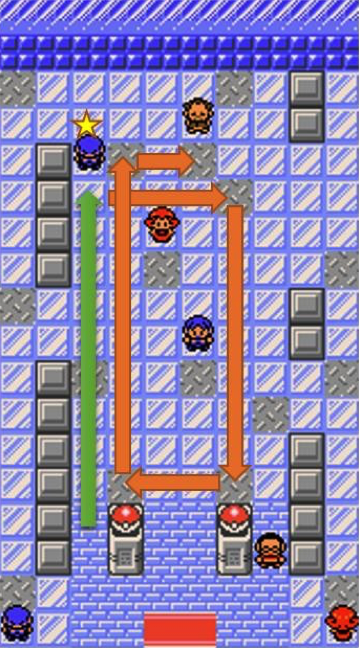
\includegraphics[scale=0.4]{../Graphics/9. Pryce's Gym.png}
	\varwe
\end{story}

\switchcolumn*
\begin{enumerate}[resume]
	\item \emphasis{Avoid spinner: Boarder Douglas (star in picture)}
\end{enumerate}

\begin{boss}{Pryce}
	\varwb
	\begin{fightSection}{Seel}
		\item \bossHl{(2)} \strength
		\begin{notes}
			\small{\item \bossHl{(3)} \bite{} \textit{(if necessary)}}
		\end{notes}
	\end{fightSection}
	\begin{fightSection}{Dewgong}
		\item \bossHl{(2)} \strength{} \bossHlTwo{2x}
		\begin{notes}
			\small{\item \bossHl{(3)} \bite{} \textit{(if necessary)}}
		\end{notes}
	\end{fightSection}
	\begin{fightSection}{Piloswine}
		\item \bossHl{(4)} \surf
	\end{fightSection}
	\varwe
\end{boss}

\begin{menu}{After Exiting the Gym}
	\varwb
	\begin{pokeMenu}
		\item \menuHlTwo{(1)} \fly{} to Olivine City \menuHlTwo{(4\pointDown)}
	\end{pokeMenu}
	\varwe
\end{menu}

\switchcolumn
\begin{trainer}{Boarder Douglas}
	\varwb
	\begin{fightSection}{Shellder/Cloyster/Shellder}
		\item \trainerHl{(3)} \bite{} \trainerHlTwo{4x}
	\end{fightSection}
	\varwe
\end{trainer}

\begin{misc}{PP Route: Pryce}
	\varwb
	\begin{tabu} to \textwidth {X[6,c] X[5,c] X[4,c] X[4,c]}
		\textbf{Headbutt/Ice Punch} & \textbf{Bite/Return} & \textbf{Surf} & \textbf{Strength}\\ 
		8 & 22 & 7 & 9
	\end{tabu}
	\varwe
\end{misc}

\begin{story}{Fly to Olivine City}
	\varwb
	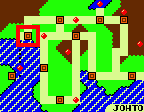
\includegraphics[scale=1.045]{../Graphics/10. Olivine City.png}
	\varwe
\end{story}

\end{paracol}
\vspace{3.5mm}
\chapter{Lighthouse}
\vspace{0.5mm}

\begin{paracol}{2}
\begin{enumerate}
	\item Head southeast to the Lighthouse and make your way back up \emphasis{(be careful of the trainer on your left after the first Gentleman)}
	\item Fall down the \emphasis{left side of the hole} past the girl and grab the \pickup{Ether}
	\item \emphasis{Avoid spinner: Sailor Ernest}
	\item \dialog{Deliver the Potion to Jasmine before leaving (hold A)}
\end{enumerate}

\switchcolumn
\begin{trainer}{Sailor Ernest}
	\varwb
	\begin{fightSection}{Machop/Machop}
		\item \trainerHl{(1)} \headbutt{} \trainerHlTwo{2x}
	\end{fightSection}
	\begin{fightSection}{Poliwhirl}
		\item \trainerHl{(3)} \bite
	\end{fightSection}
	\varwe
\end{trainer}

\switchcolumn
\begin{menu}{After Delivering the Potion}
	\varwb
	\begin{packMenu}
		\item \escapeRope
	\end{packMenu}
	\varwe
\end{menu}

\switchcolumn*
\begin{misc}{PP Route: Jasmine}
	\varwb
	\begin{tabu} to \textwidth {X[6,c] X[5,c] X[4,c] X[4,c]}
		\textbf{Headbutt/Ice Punch} & \textbf{Bite/Return} & \textbf{Surf} & \textbf{Strength}\\ 
		8 & 22 & 4 & 9
	\end{tabu}
	\varwe
\end{misc}

\switchcolumn
\begin{enumerate}[resume]
	\item Head northwest to the Gym
\end{enumerate}

\begin{boss}{Jasmine}
	\varwb
	\begin{fightSection}{Magnemite/Magnemite/Steelix}
		\item \bossHl{(4)} \surf{} \bossHlTwo{3x}
	\end{fightSection}
	\varwe
\end{boss}

\begin{menu}{After Exiting the Gym}
	\varwb
	\begin{pokeMenu}
		\item \menuHlTwo{(1)} \fly{} to Goldenrod City \menuHlTwo{(4\pointUp)}
	\end{pokeMenu}
	\varwe
\end{menu}

\switchcolumn
\begin{story}{Fly to Goldenrod City}
	\varwb
	\insertMap{../Graphics/11. Goldenrod City.png}
	\varwe
\end{story}

\end{paracol}
\vspace{3.5mm}
\chapter{Radio Tower}
\vspace{0.5mm}

\begin{paracol}{2}
\begin{enumerate}
    \item \emphasis{Heal at the Pokemon Center if you hit both Douglas and Ernest}
    \item Head east to the Mart
\end{enumerate}

\begin{shop}{Goldenrod City Mart}
	\varwb
	\begin{notes}
		\item \textbf{Floor 5 (right clerk)}
		\item \shopHlThree{Get TM27 (Return) from the left clerk}
		\begin{buy}
            \item \shopHl{(2\pointDown)} TM33 (Ice Punch)
        \end{buy}
	\end{notes}
	\begin{notes}
		\item \textbf{Floor 4}
		\item \shopHlThree{Only if 10-12 DV SPC}
		\begin{buy}
            \item \shopHl{(3\pointDown)} \calcium{} \shopHlTwo{2x}
        \end{buy}
	\end{notes}
    \begin{notes}
		\item \textbf{Floor 3}
		\begin{buy}
            \item \shopHl{(\pointDown)} \xSpecial{} \shopHlTwo{6x}
            \item \shopHl{(2\pointDown)} \xAttack{} \shopHlTwo{11x}
            \item \shopHl{(3\pointUp)} \xSpeed{} \shopHlTwo{3x}
            \begin{notes}
                \small{\item \shopHlThree{2x} \textbf{(if $>$10 DV SPD)}}
            \end{notes}
            \item \shopHl{(5\pointDown)} \guardSpec{}
            \item \shopHl{(\pointDown)} \xAccuracy{} \shopHlTwo{3x}
        \end{buy}
	\end{notes}
	\varwe
\end{shop}

\begin{enumerate}[resume]
    \item Head northwest to the Radio Tower
\end{enumerate}

\switchcolumn*
\alignBoxes
\begin{misc}{PP Route: Rocket Grunt \#1}
	\varwb
	\begin{tabu} to \textwidth {X[6,c] X[5,c] X[4,c] X[4,c]}
		\textbf{Headbutt/Ice Punch} & \textbf{Bite/Return} & \textbf{Surf} & \textbf{Strength}\\ 
		6 & 22 & 4 & 9
	\end{tabu}
	\varwe
\end{misc}

\begin{misc}{When You Hit L38}
	\varwb
	\begin{notes}
		\item \emphasis{B \pointRight{} A to cancel learning Slash}
	\end{notes}
	\varwe
\end{misc}

\switchcolumn
\begin{trainer}{Rocket Grunt \#1}
	\varwb
	\begin{fightSection}{Raticate/Raticate}
		\item \trainerHl{(1)} \headbutt{} \trainerHlTwo{2x}
	\end{fightSection}
	\varwe
\end{trainer}

\begin{enumerate}[resume]
    \item On the second floor: go down \pointRight{} around \pointRight{} up between the two Grunts
\end{enumerate}

\switchcolumnTwice[*]
\begin{trainer}{Rocket Grunt \#2}
	\varwb
	\begin{fightSection}{Zubat/Zubat}
		\item \trainerHl{(1)} \headbutt{} \trainerHlTwo{2x}
	\end{fightSection}
	\varwe
\end{trainer}

\switchcolumn
\begin{misc}{PP Route: Rocket Grunt \#2}
	\varwb
	\begin{tabu} to \textwidth {X[6,c] X[5,c] X[4,c] X[4,c]}
		\textbf{Headbutt/Ice Punch} & \textbf{Bite/Return} & \textbf{Surf} & \textbf{Strength}\\ 
		4 & 22 & 4 & 9
	\end{tabu}
	\varwe
\end{misc}

\begin{misc}{PP Route: Rocket Grunt \#3}
	\varwb
	\begin{tabu} to \textwidth {X[6,c] X[5,c] X[4,c] X[4,c]}
		\textbf{Headbutt/Ice Punch} & \textbf{Bite/Return} & \textbf{Surf} & \textbf{Strength}\\ 
		0 & 22 & 4 & 9
	\end{tabu}
	\varwe
\end{misc}

\switchcolumn
\begin{trainer}{Rocket Grunt \#3}
	\varwb
	\begin{fightSection}{Grimer/Grimer/Muk}
		\item \trainerHl{(1)} \headbutt{} \trainerHlTwo{4x}
	\end{fightSection}
	\varwe
\end{trainer}

\begin{enumerate}[resume]
    \item On Floor 3 go straight right to \dialog{the Grunt on the north wall and speak to him}
\end{enumerate}

\switchcolumn*
\begin{misc}{PP Route: Rocket Grunt \#4}
	\varwb
	\begin{tabu} to \textwidth {X[6,c] X[5,c] X[4,c] X[4,c]}
		\textbf{Headbutt/Ice Punch} & \textbf{Bite/Return} & \textbf{Surf} & \textbf{Strength}\\ 
		0 & 19 & 4 & 8
	\end{tabu}
	\varwe
\end{misc}

\switchcolumn
\begin{trainer}{Rocket Grunt \#4}
	\varwb
	\begin{fightSection}{Koffing}
		\item \trainerHl{(3)} \bite
	\end{fightSection}
	\begin{fightSection}{Grimer}
		\item \trainerHl{(2)} \strength
	\end{fightSection}
	\begin{fightSection}{Zubat/Rattata}
		\item \trainerHl{(3)} \bite{} \trainerHlTwo{2x}
	\end{fightSection}
	\varwe
\end{trainer}

\begin{enumerate}[resume]
    \item Go down and left to the south wall
    \item \dialog{Talk to the Scientist on the right}
\end{enumerate}

\switchcolumn*
\begin{misc}{PP Route: Scientist Marc}
	\varwb
	\begin{tabu} to \textwidth {X[6,c] X[5,c] X[4,c] X[4,c]}
		\textbf{Headbutt/Ice Punch} & \textbf{Bite/Return} & \textbf{Surf} & \textbf{Strength}\\ 
		0 & 19 & 1 & 8
	\end{tabu}
	\varwe
\end{misc}

\switchcolumn
\begin{trainer}{Scientist Marc}
	\varwb
	\begin{fightSection}{Magnemite/Magnemite/Magnemite}
		\item \trainerHl{(4)} \surf{} \trainerHlTwo{3x}
	\end{fightSection}
	\varwe
\end{trainer}

\begin{enumerate}[resume]
    \item Head up to floor 4 and \emphasis{avoid rotator}
\end{enumerate}

\begin{menu}{Before the Next Fights}
	\varwb
	\begin{packMenu}
		\item \ether{} \pointRight{} \surf{} \menuHlTwo{(4)}
		\item \calcium{} \textit{(if you bought them)}
		\item \menuHlTwo{(\pointLeft{})} \textbf{\#33 \icePunch{}} \switch{} \headbutt{} \menuHlTwo{(1)}
	\end{packMenu}
	\varwe
\end{menu}

\switchcolumn*
\begin{misc}{PP Route: Scientist Rich}
	\varwb
	\begin{tabu} to \textwidth {X[6,c] X[5,c] X[4,c] X[4,c]}
		\textbf{Headbutt/Ice Punch} & \textbf{Bite/Return} & \textbf{Surf} & \textbf{Strength}\\ 
		15 & 18 & 10 & 8
	\end{tabu}
	\varwe
\end{misc}

\switchcolumn
\begin{trainer}{Scientist Rich}
	\varwb
	\begin{fightSection}{Porygon}
		\item \trainerHl{(4)} \surf
		\item \trainerHl{(3)} \bite
	\end{fightSection}
	\varwe
\end{trainer}

\switchcolumn*
\begin{misc}{PP Route: Rocket Executive}
	\varwb
	\begin{tabu} to \textwidth {X[6,c] X[5,c] X[4,c] X[4,c]}
		\textbf{Headbutt/Ice Punch} & \textbf{Bite/Return} & \textbf{Surf} & \textbf{Strength}\\ 
		15 & 14 & 8 & 8
	\end{tabu}
	\varwe
\end{misc}

\switchcolumn
\begin{trainer}{Rocket Executive}
	\varwb
	\begin{fightSection}{Koffing}
		\item \trainerHl{(4)} \surf
	\end{fightSection}
	\begin{fightSection}{Koffing}
		\item \xSpecial
		\item \trainerHl{(3)} \bite
	\end{fightSection}
	\begin{fightSection}{Koffing}
		\item \trainerHl{(3)} \bite
	\end{fightSection}
	\begin{fightSection}{Weezing}
		\item \trainerHl{(4)} \surf
	\end{fightSection}
	\begin{fightSection}{Koffing/Koffing}
		\item \trainerSwap{\textbf{(4)} \surf{} \switch{} \textbf{(3)} \bite}
		\item \trainerHl{(4)} \bite{} \trainerHlTwo{2x}
	\end{fightSection}
	\varwe
\end{trainer}

\begin{enumerate}[resume]
    \item Walk out of the Radio Tower and \emphasis{avoid rotator (you can still get trainer battles)}
    \item Enter Underground via the small northwest building
\end{enumerate}

\end{paracol}
\vspace{3.5mm}
\chapter{Underground}
\vspace{0.5mm}

\begin{paracol}{2}

\begin{enumerate}
	\item Enter the door on the east side
\end{enumerate}

\switchcolumn*
\alignBoxes
\begin{misc}{PP Route: Rival \#3}
	\varwb
	\begin{tabu} to \textwidth {X[6,c] X[5,c] X[4,c] X[4,c]}
		\textbf{Headbutt/Ice Punch} & \textbf{Bite/Return} & \textbf{Surf} & \textbf{Strength}\\ 
		12 & 14 & 6 & 8
	\end{tabu}
	\varwe
\end{misc}

\begin{menu}{Conditional Menu After Rival \#3}
	\varwb
	\begin{packMenu}
		\item \fullHeal{} \emphasis{(if \poison[ed])}
	\end{packMenu}
	\varwe
\end{menu}

\switchcolumn
\begin{boss}{Rival \#3}
	\varwb
	\begin{fightSection}{Golbat}
		\item \bossHl{(1)} \icePunch
	\end{fightSection}
	\begin{fightSection}{Magenemite}
		\item \bossNote{\textbf{\xSpecial{}} \textit{(if PRZCureBerry)}}
		\item \bossHl{(3)} \surf
	\end{fightSection}
	\begin{fightSection}{Meganium}
		\item \bossNote{\textbf{\xSpecial{}} \textit{(otherwise)}}
		\item \bossHl{(1)} \icePunch
	\end{fightSection}
	\begin{fightSection}{Haunter}
		\item \bossHl{(1)} \icePunch
	\end{fightSection}
	\begin{fightSection}{Sneasel}
		\item \bossHl{(3)} \surf
	\end{fightSection}
	\varwe
\end{boss}

\switchcolumn*
\begin{misc}{PP Route: Rocket Grunt \#1}
	\varwb
	\begin{tabu} to \textwidth {X[6,c] X[5,c] X[4,c] X[4,c]}
		\textbf{Headbutt/Ice Punch} & \textbf{Bite/Return} & \textbf{Surf} & \textbf{Strength}\\ 
		12 & 13 & 6 & 8
	\end{tabu}
	\varwe
\end{misc}

\switchcolumn
\begin{trainer}{Rocket Grunt \#1}
	\varwb
	\begin{fightSection}{Rattata}
		\item \bossSwap{\textbf{(1)} \icePunch{} \switch{} \textbf{(4)} \bite}
		\item \trainerHl{(1)} \bite
	\end{fightSection}
	\varwe
\end{trainer}

\switchcolumn*
\begin{misc}{PP Route: Rocket Grunt \#2}
	\varwb
	\begin{tabu} to \textwidth {X[6,c] X[5,c] X[4,c] X[4,c]}
		\textbf{Headbutt/Ice Punch} & \textbf{Bite/Return} & \textbf{Surf} & \textbf{Strength}\\ 
		12 & 11 & 5 & 8
	\end{tabu}
	\varwe
\end{misc}

\switchcolumn
\begin{trainer}{Rocket Grunt \#2}
	\varwb
	\begin{fightSection}{Muk}
		\item \trainerHl{(3)} \surf
		\begin{notes}
			\small{\item \trainerHl{(1)} \bite{} \textit{(if necessary)}}
		\end{notes}
	\end{fightSection}
	\begin{fightSection}{Koffing/Rattata}
		\item \trainerHl{(1)} \bite{} \trainerHlTwo{2x}
	\end{fightSection}
	\varwe
\end{trainer}

\switchcolumn*
\begin{misc}{PP Route: Rocket Grunt \#3}
	\varwb
	\begin{tabu} to \textwidth {X[6,c] X[5,c] X[4,c] X[4,c]}
		\textbf{Headbutt/Ice Punch} & \textbf{Bite/Return} & \textbf{Surf} & \textbf{Strength}\\ 
		12 & 10 & 4 & 8
	\end{tabu}
	\varwe
\end{misc}

\switchcolumn
\begin{trainer}{Rocket Grunt \#3}
	\varwb
	\begin{fightSection}{Koffing}
		\item \trainerHl{(1)} \bite
	\end{fightSection}
	\begin{fightSection}{Muk}
		\item \trainerHl{(3)} \surf
		\begin{notes}
			\small{\item \trainerHl{(1)} \bite{} \textit{(if necessary)}}
		\end{notes}
	\end{fightSection}
	\varwe
\end{trainer}

\begin{enumerate}[resume]
	\item Hit switches from left to right: \textbf{3 \pointRight{} 2 \pointRight{} 1}
\end{enumerate}

\switchcolumn
\newpage
\begin{misc}{PP Route: Burglar Eddie}
	\varwb
	\begin{tabu} to \textwidth {X[6,c] X[5,c] X[4,c] X[4,c]}
		\textbf{Headbutt/Ice Punch} & \textbf{Bite/Return} & \textbf{Surf} & \textbf{Strength}\\ 
		12 & 9 & 4 & 7
	\end{tabu}
	\varwe
\end{misc}

\switchcolumn
\newpage
\begin{trainer}{Burglar Eddie}
	\varwb
	\begin{fightSection}{Growlithe}
		\item \trainerHl{(2)} \strength
	\end{fightSection}
	\begin{fightSection}{Koffing}
		\item \trainerHl{(1)} \bite
	\end{fightSection}
	\varwe
\end{trainer}

\switchcolumn*
\begin{misc}{PP Route: Burglar Duncan}
	\varwb
	\begin{tabu} to \textwidth {X[6,c] X[5,c] X[4,c] X[4,c]}
		\textbf{Headbutt/Ice Punch} & \textbf{Bite/Return} & \textbf{Surf} & \textbf{Strength}\\ 
		12 & 7 & 4 & 6
	\end{tabu}
	\varwe
\end{misc}

\switchcolumn
\begin{trainer}{Burglar Duncan}
	\varwb
	\begin{fightSection}{Koffing/Koffing}
		\item \trainerHl{(1)} \bite{} \trainerHlTwo{2x}
	\end{fightSection}
	\begin{fightSection}{Magmar}
		\item \trainerHl{(2)} \strength
	\end{fightSection}
	\varwe
\end{trainer}

\switchcolumn*
\begin{misc}{PP Route: Rocket Grunt \#4}
	\varwb
	\begin{tabu} to \textwidth {X[6,c] X[5,c] X[4,c] X[4,c]}
		\textbf{Headbutt/Ice Punch} & \textbf{Bite/Return} & \textbf{Surf} & \textbf{Strength}\\ 
		12 & 7 & 4 & 4
	\end{tabu}
	\varwe
\end{misc}

\switchcolumn
\begin{trainer}{Rocket Grunt \#4}
	\varwb
	\begin{fightSection}{Gloom/Gloom}
		\item \trainerHl{(2)} \strength{} \trainerHlTwo{2x}
	\end{fightSection}
	\varwe
\end{trainer}

\begin{enumerate}[resume]
	\item \emphasis{Do not hit the switch}
\end{enumerate}

\switchcolumn*
\begin{misc}{PP Route: Rocket Grunt \#5}
	\varwb
	\begin{tabu} to \textwidth {X[6,c] X[5,c] X[4,c] X[4,c]}
		\textbf{Headbutt/Ice Punch} & \textbf{Bite/Return} & \textbf{Surf} & \textbf{Strength}\\ 
		11 & 7 & 4 & 3
	\end{tabu}
	\varwe
\end{misc}

\switchcolumn
\begin{trainer}{Rocket Grunt \#5}
	\varwb
	\begin{fightSection}{Raticate}
		\item \trainerHl{(4)} \icePunch
	\end{fightSection}
	\begin{fightSection}{Golbat}
		\item \trainerHl{(2)} \strength
	\end{fightSection}
	\varwe
\end{trainer}

\switchcolumn*
\begin{misc}{PP Route: Rocket Grunt \#6}
	\varwb
	\begin{tabu} to \textwidth {X[6,c] X[5,c] X[4,c] X[4,c]}
		\textbf{Headbutt/Ice Punch} & \textbf{Bite/Return} & \textbf{Surf} & \textbf{Strength}\\ 
		10 & 7 & 4 & 2
	\end{tabu}
	\varwe
\end{misc}

\switchcolumn
\begin{trainer}{Rocket Grunt \#6}
	\varwb
	\begin{fightSection}{Grimer}
		\item \trainerHl{(2)} \strength
	\end{fightSection}
	\begin{fightSection}{Weezing}
		\item \trainerHl{(4)} \icePunch
	\end{fightSection}
	\varwe
\end{trainer}

\begin{enumerate}[resume]
	\item \emphasis{Do not go up the stairs}
\end{enumerate}

\switchcolumn*
\begin{misc}{PP Route: Rocket Grunt \#7}
	\varwb
	\begin{tabu} to \textwidth {X[6,c] X[5,c] X[4,c] X[4,c]}
		\textbf{Headbutt/Ice Punch} & \textbf{Bite/Return} & \textbf{Surf} & \textbf{Strength}\\ 
		10 & 5 & 4 & 2
	\end{tabu}
	\varwe
\end{misc}

\switchcolumn
\begin{trainer}{Rocket Grunt \#7}
	\varwb
	\begin{fightSection}{Koffing/Koffing}
		\item \trainerHl{(1)} \bite{} \trainerHlTwo{2x}
	\end{fightSection}
	\varwe
\end{trainer}

\begin{enumerate}[resume]
	\item \dialog{Get the Card Key from the Director}
\end{enumerate}

\begin{menu}{After Getting the Card Key}
	\varwb
	\begin{packMenu}
		\item \menuHlTwo{(\pointLeft{})} \textbf{\#27 \return{}} \switch{} \bite{} \menuHlTwo{(1)}
		\item \escapeRope
	\end{packMenu}
	\varwe
\end{menu}

\begin{enumerate}[resume]
	\item Head southwest back to the Radio Tower
	\item Head up to the third floor and use the Card Key \emphasis{(you can still get trainer battles)}
\end{enumerate}

\switchcolumn*
\begin{misc}{PP Route: Rocket Grunt \#1}
	\varwb
	\begin{tabu} to \textwidth {X[6,c] X[5,c] X[4,c] X[4,c]}
		\textbf{Headbutt/Ice Punch} & \textbf{Bite/Return} & \textbf{Surf} & \textbf{Strength}\\ 
		9 & 19 & 4 & 2
	\end{tabu}
	\varwe
\end{misc}

\switchcolumn
\begin{trainer}{Rocket Grunt \#1}
	\varwb
	\begin{fightSection}{Raticate/Koffing}
		\item \trainerHl{(4)} \icePunch{} \trainerHlTwo{2x}
	\end{fightSection}
	\varwe
\end{trainer}

\switchcolumn
\begin{misc}{PP Route: Rocket Executive \#1}
	\varwb
	\begin{tabu} to \textwidth {X[6,c] X[5,c] X[4,c] X[4,c]}
		\textbf{Headbutt/Ice Punch} & \textbf{Bite/Return} & \textbf{Surf} & \textbf{Strength}\\ 
		8 & 19 & 4 & 2
	\end{tabu}
	\varwe
\end{misc}

\switchcolumn
\begin{trainer}{Rocket Executive \#1}
	\varwb
	\begin{fightSection}{Golbat}
		\item \trainerHl{(4)} \icePunch
		\begin{notes}
			\small{\item \trainerHl{(1)} \return{} \textit{(if necessary)}}
		\end{notes}
	\end{fightSection}
	\varwe
\end{trainer}

\begin{enumerate}[resume]
	\item Head upstairs
\end{enumerate}

\switchcolumn*
\begin{misc}{PP Route: Rocket Executive \#2}
	\varwb
	\begin{tabu} to \textwidth {X[6,c] X[5,c] X[4,c] X[4,c]}
		\textbf{Headbutt/Ice Punch} & \textbf{Bite/Return} & \textbf{Surf} & \textbf{Strength}\\ 
		7 & 18 & 3 & 2
	\end{tabu}
	\varwe
\end{misc}

\switchcolumn
\begin{trainer}{Rocket Executive \#2}
	\varwb
	\begin{fightSection}{Arbok}
		\item \trainerHl{(3)} \surf
		\begin{notes}
			\small{\item \trainerHl{(1)} \return{} \textit{(if necessary)}}
		\end{notes}
	\end{fightSection}
	\begin{fightSection}{Vileplume}
		\item \trainerHl{(4)} \icePunch
		\begin{notes}
			\small{\item \trainerHl{(1)} \return{} \textit{(if necessary)}}
		\end{notes}
	\end{fightSection}
	\begin{fightSection}{Murkrow}
		\item \trainerHl{(1)} \return
	\end{fightSection}
	\varwe
\end{trainer}

\switchcolumn*
\begin{misc}{PP Route: Rocket Executive \#3}
	\varwb
	\begin{tabu} to \textwidth {X[6,c] X[5,c] X[4,c] X[4,c]}
		\textbf{Headbutt/Ice Punch} & \textbf{Bite/Return} & \textbf{Surf} & \textbf{Strength}\\ 
		6 & 17 & 2 & 2
	\end{tabu}
	\varwe
\end{misc}

\switchcolumn
\begin{trainer}{Rocket Executive \#3}
	\varwb
	\begin{fightSection}{Houndour}
		\item \trainerHl{(1)} \return
	\end{fightSection}
	\begin{fightSection}{Koffing}
		\item \trainerHl{(4)} \icePunch
	\end{fightSection}
	\begin{fightSection}{Houndoom}
		\item \trainerHl{(3)} \surf
	\end{fightSection}
	\varwe
\end{trainer}

\switchcolumn*
\vspace{-2mm}
\begin{story}{Fly to Mahogany Town}
	\varwb
	\insertMap{../Graphics/8. Mahogany Town.png}
	\varwe
\end{story}

\switchcolumn
\begin{enumerate}[resume]
	\item \dialog{Get the Pink Bow from Mary one floor below}
	\item Walk to the bottom floor
	\item \dialog{Talk to the right lady behind the counter to take the quiz (Yes)}
	\item Quiz answers: \textbf{Yes \pointRight{} Yes \pointRight{} No \pointRight{} Yes \pointRight{} No}
\end{enumerate}

\begin{menu}{After Exiting the Radio Tower}
	\varwb
	\begin{pokeMenu}
		\item \menuHlTwo{(1)} \fly{} to Mahogany Town \menuHlTwo{(2\pointDown)}
	\end{pokeMenu}
	\varwe
\end{menu}

\newpage
\end{paracol}
\vspace{3.5mm}
\chapter{Ice Path}
\vspace{0.5mm}

\begin{paracol}{2}
\begin{enumerate}
	\item Head east out of Mahogany Town and \emphasis{avoid rotator}
	\item \emphasis{Bike along the bottom row until the girl}
	\item \emphasis{Bike along the top row to avoid the next trainer}
\end{enumerate}

\switchcolumn
\begin{misc}{PP Route: Bird Keeper Vance}
	\varwb
	\begin{tabu} to \textwidth {X[6,c] X[5,c] X[4,c] X[4,c]}
		\textbf{Headbutt/Ice Punch} & \textbf{Bite/Return} & \textbf{Surf} & \textbf{Strength}\\ 
		6 & 17 & 2 & 0
	\end{tabu}
	\varwe
\end{misc}

\switchcolumn
\begin{trainer}{Bird Keeper Vance}
	\varwb
	\begin{fightSection}{Pidgeotto/Pidgeotto}
		\item \trainerHl{(2)} \strength{} \trainerHlTwo{2x}
	\end{fightSection}
	\varwe
\end{trainer}

\begin{menu}{After Entering the Ice Path}
	\varwb
	\begin{packMenu}
		\item \superRepel
	\end{packMenu}
	\varwe
\end{menu}

\begin{enumerate}[resume]
	\item Do the Ice Path puzzle \emphasis{(right image)} and grab \pickup{HM07 (Waterfall)}
\end{enumerate}

\switchcolumn
\begin{story}{Ice Path Puzzle}
	\varwb
	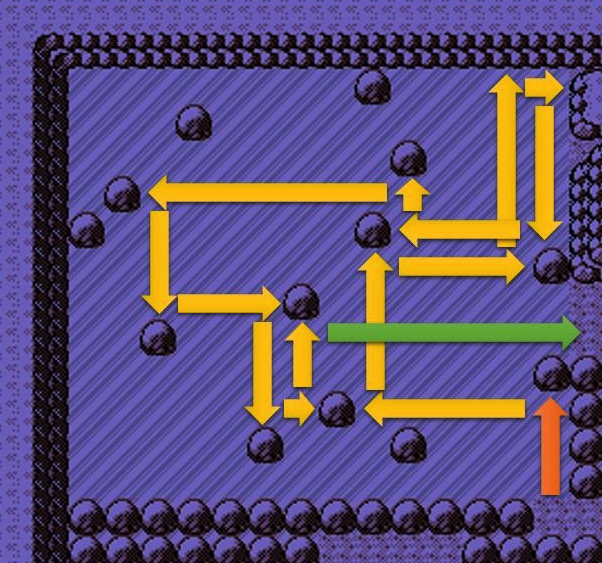
\includegraphics[scale=0.4]{../Graphics/12. Ice Path 1.png}
	\varwe
\end{story}

\switchcolumn
\begin{story}{Getting HM07}
	\varwb
	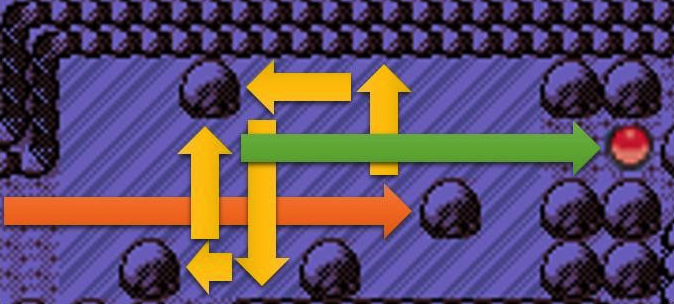
\includegraphics[scale=0.25]{../Graphics/13. Ice Path 2.png}
	\varwe
\end{story}

\begin{enumerate}[resume]
	\item Follow \emphasis{image \#1} and end with knocking boulder \#1 down the hole
	\item Leave the room via the southwest hole
	\item Bike up \pointRight{} right \pointRight{} down the ladder
	\item Jump off the ledge \emphasis{on the left side} \pointRight{} down \pointRight{} left \pointRight{} into the ladder \emphasis{(image \#2)}
	\item Go around to the ice and follow this path: \textbf{down \pointRight{} right \pointRight{} up \pointRight{} left \pointRight{} up \pointRight{} left \pointRight{} down \pointRight{} left}
	\item In the next room, jump off the ledge and exit the cave \emphasis{(image \#3)}
\end{enumerate}

\begin{story}{Boulder Puzzle \#1}
	\varwb
	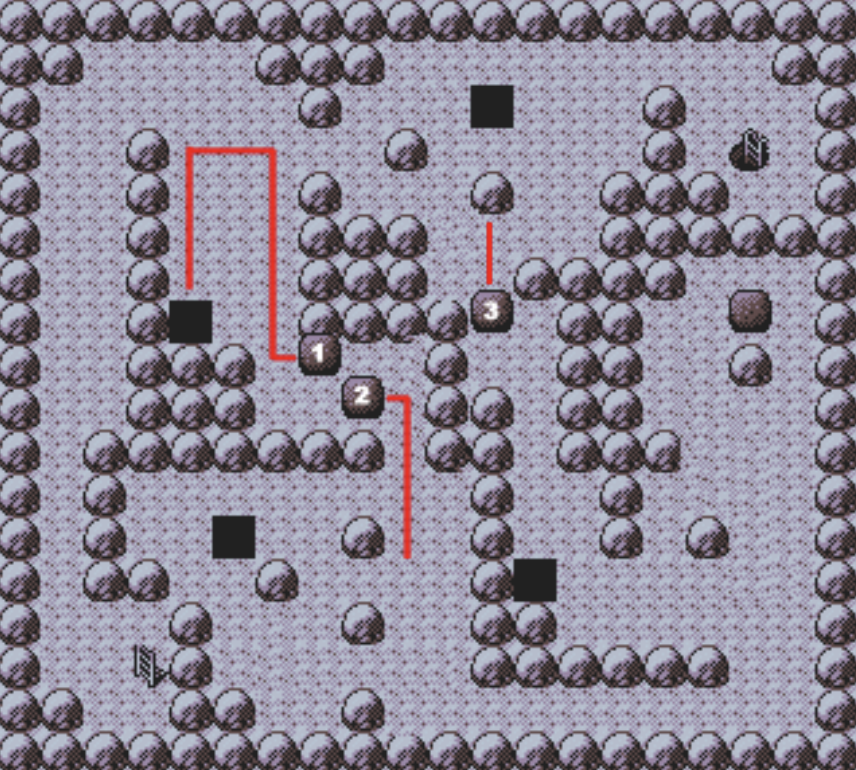
\includegraphics[scale=0.65]{../Graphics/14. Boulder Puzzle 1.png}
	\varwe
\end{story}

\switchcolumn
\begin{menu}{When Repel Runs Out}
	\varwb
	\begin{packMenu}
		\item \superRepel
	\end{packMenu}
	\begin{pokeMenu}
		\item \menuHlTwo{(1)} \strength
	\end{pokeMenu}
	\varwe
\end{menu}

\begin{story}{Boulder Puzzle \#2}
	\varwb
	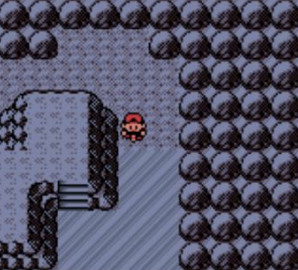
\includegraphics{../Graphics/15. Boulder Puzzle 2.png}
	\varwe
\end{story}

\begin{story}{Boulder Puzzle \#3}
	\varwb
	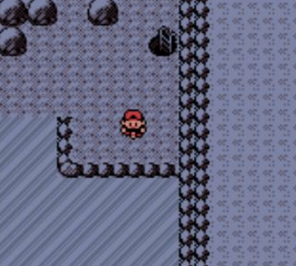
\includegraphics{../Graphics/16. Boulder Puzzle 3.png}
	\varwe
\end{story}

\end{paracol}
\vspace{3.5mm}
\chapter{Blackthorn City}
\vspace{0.5mm}

\begin{paracol}{2}
\begin{enumerate}
	\item After exiting the cave, head south \pointRight{} west \pointRight{} north to get to the Gym
\end{enumerate}

\begin{menu}{At the Sign}
	\varwb
	\begin{packMenu}
		\item \superRepel
		\small{\item \superPotion{} \textit{(if necessary)}}
		\item \textbf{\pinkBow{}} \pointRight{} Give \menuHlTwo{(1)}
		\item \menuHlTwo{(\pointLeft{})} H6 \whirlpool{} \menuHlTwo{(1)}
		\item \menuHlTwo{(\pointLeft{})} H7 \waterfall{} \menuHlTwo{(4)}
	\end{packMenu}
	\varwe
\end{menu}

\switchcolumn*
\alignBoxes
\begin{misc}{PP Route: Cooltrainer Paul}
	\varwb
	\begin{tabu} to \textwidth {X[6,c] X[5,c] X[4,c] X[4,c]}
		\textbf{Headbutt/Ice Punch} & \textbf{Bite/Return} & \textbf{Surf} & \textbf{Strength}\\ 
		6 & 14 & 2 & 0
	\end{tabu}
	\varwe
\end{misc}

\switchcolumn
\begin{trainer}{Cooltrainer Paul}
	\varwb
	\begin{fightSection}{Dratini/Dratini/Dratini}
		\item \trainerHl{(1)} \return{} \trainerHlTwo{3x}
	\end{fightSection}
	\varwe
\end{trainer}

\switchcolumn*
\begin{misc}{PP Route: Cooltrainer Fran}
	\varwb
	\begin{tabu} to \textwidth {X[6,c] X[5,c] X[4,c] X[4,c]}
		\textbf{Headbutt/Ice Punch} & \textbf{Bite/Return} & \textbf{Surf} & \textbf{Strength}\\ 
		6 & 12 & 2 & 0
	\end{tabu}
	\varwe
\end{misc}

\switchcolumn
\begin{trainer}{Cooltrainer Fran}
	\varwb
	\begin{fightSection}{Seadra}
		\item \trainerHl{(1)} \return{} \trainerHlTwo{2x}
	\end{fightSection}
	\varwe
\end{trainer}

\begin{enumerate}[resume]
	\item Push bottom-right boulder down \pointRight{} bottom-left rock up and into the hole near the stairs
	\item Continue north to the next trainer
\end{enumerate}

\switchcolumn*
\begin{misc}{PP Route: Cooltrainer Cody}
	\varwb
	\begin{tabu} to \textwidth {X[6,c] X[5,c] X[4,c] X[4,c]}
		\textbf{Headbutt/Ice Punch} & \textbf{Bite/Return} & \textbf{Surf} & \textbf{Strength}\\ 
		6 & 9 & 2 & 0
	\end{tabu}
	\varwe
\end{misc}

\switchcolumn
\begin{trainer}{Cooltrainer Cody}
	\varwb
	\begin{fightSection}{Horsea/Seadra}
		\item \trainerHl{(1)} \return{} \trainerHlTwo{3x}
	\end{fightSection}
	\varwe
\end{trainer}

\begin{enumerate}[resume]
	\item Push the right boulder into the wall \pointRight{} push the other boulder down the hole
	\item Jump down the hole then head northeast to the next trainer
\end{enumerate}

\switchcolumn*
\begin{misc}{PP Route: Cooltrainer Lola}
	\varwb
	\begin{tabu} to \textwidth {X[6,c] X[5,c] X[4,c] X[4,c]}
		\textbf{Headbutt/Ice Punch} & \textbf{Bite/Return} & \textbf{Surf} & \textbf{Strength}\\ 
		5 & 8 & 2 & 0
	\end{tabu}
	\varwe
\end{misc}

\switchcolumn
\begin{trainer}{Cooltrainer Lola}
	\varwb
	\begin{fightSection}{Dratini}
		\item \trainerHl{(1)} \return
	\end{fightSection}
	\begin{fightSection}{Dragonair}
		\item \trainerHl{(4)} \icePunch
	\end{fightSection}
	\varwe
\end{trainer}

\switchcolumn*
\begin{misc}{PP Route: Clair}
	\varwb
	\begin{tabu} to \textwidth {X[6,c] X[5,c] X[4,c] X[4,c]}
		\textbf{Headbutt/Ice Punch} & \textbf{Bite/Return} & \textbf{Surf} & \textbf{Strength}\\ 
		2 & 6 & 2 & 0
	\end{tabu}
	\varwe
\end{misc}

\begin{misc}{If You Hit L47}
	\varwb
	\begin{notes}
		\item \emphasis{B \pointRight{} A to cancel learning Screech}
	\end{notes}
	\varwe
\end{misc}

\switchcolumn
\begin{boss}{Clair}
	\varwb
	\begin{fightSection}{Dragonair/Dragonair/Dragonair}
		\item \bossHl{(4)} \icePunch{} \bossHlTwo{3x}
	\end{fightSection}
	\begin{fightSection}{Kingdra}
		\item \bossHl{(1)} \return{} \bossHlTwo{2x}
	\end{fightSection}
	\varwe
\end{boss}

\begin{enumerate}[resume]
	\item Exit and Surf to Dragon's Den behind the Gym
	\item Follow the path \pointRight{} when outside again keep heading left until you can't anymore
	\item Head south and use Whirlpool
	\item Continue around and up on the other side to get the \pickup{Dragon Fang}
\end{enumerate}

\switchcolumn*
\vspace{-0.8cm}
\begin{story}{Fly to New Bark Town}
	\varwb
	\insertMap{../Graphics/17. New Bark Town.png}
	\varwe
\end{story}

\switchcolumn
\begin{menu}{After Getting the Rising Badge}
	\varwb
	\begin{packMenu}
		\item \superRepel
		\item \escapeRope
	\end{packMenu}
	\varwe
\end{menu}

\begin{menu}{After Using the Escape Rope}
	\varwb
	\begin{pokeMenu}
		\item \menuHlTwo{(1)} \fly{} to New Bark Town \menuHlTwo{(A)}
	\end{pokeMenu}
	\varwe
\end{menu}

\end{paracol}
\vspace{3.5mm}
\chapter{Victory Road}
\vspace{0.5mm}

\begin{paracol}{2}
\begin{enumerate}
	\item Surf east and enter the cave on the other side
	\item Head up the waterfall and exit the cave \emphasis{(move down immediately after exiting)}
	\item \emphasis{Avoid rotator and Surf east onto the grass}
\end{enumerate}

\switchcolumn*
\alignBoxes
\begin{misc}{PP Route: Cooltrainer Blake}
	\varwb
	\begin{tabu} to \textwidth {X[6,c] X[5,c] X[4,c] X[4,c]}
		\textbf{Headbutt/Ice Punch} & \textbf{Bite/Return} & \textbf{Surf} & \textbf{Strength}\\ 
		2 & 5 & 0 & 0
	\end{tabu}
	\varwe
\end{misc}

\begin{misc}{If You Hit L47}
	\varwb
	\begin{notes}
		\item \emphasis{B \pointRight{} A to cancel learning Screech}
	\end{notes}
	\varwe
\end{misc}

\switchcolumn
\begin{trainer}{Cooltrainer Blake}
	\varwb
	\begin{fightSection}{Magneton}
		\item \trainerHl{(3)} \surf
	\end{fightSection}
	\begin{fightSection}{Exeggcute}
		\item \trainerHl{(1)} \return
		\begin{notes}
			\small{\item \trainerHl{(4)} \icePunch{} \textit{(if only 1x Return left)}}
		\end{notes}
	\end{fightSection}
	\begin{fightSection}{Quagsire}
		\item \trainerHl{(3)} \surf
	\end{fightSection}
	\varwe
\end{trainer}

\switchcolumn
\begin{menu}{When Repel Runs Out}
	\varwb
	\begin{packMenu}
		\item \superRepel
	\end{packMenu}
	\varwe
\end{menu}

\switchcolumn
\begin{enumerate}[resume]
	\item Head right \emphasis{on the lower tile}
	\item \emphasis{Immediately surf south when you can}
	\item Head east and get back on land after the female trainer
	\item Continue and Surf again to avoid the next trainer
\end{enumerate}

\switchcolumn
\begin{misc}{PP Route: Psychic Richard (Route Ends Here)}
	\varwb
	\begin{tabu} to \textwidth {X[6,c] X[5,c] X[4,c] X[4,c]}
		\textbf{Headbutt/Ice Punch} & \textbf{Bite/Return} & \textbf{Surf} & \textbf{Strength}\\ 
		2 & 4 & 0 & 0
	\end{tabu}
	\varwe
\end{misc}

\begin{misc}{PP Management Until Kanto}
	\begin{notes}
		\item \emphasis{Only use the allotted number of Surfs}
		\item One extra cast if you don't use Surf on Beth ($\geq$13 DV ATK)
	\end{notes}
\end{misc}

\switchcolumn
\begin{trainer}{Psychic Richard}
	\varwb
	\begin{fightSection}{Espeon}
		\item \trainerHl{(1)} \return
	\end{fightSection}
	\varwe
\end{trainer}

\begin{enumerate}[resume]
	\item Continue north and enter the house
	\item \emphasis{Talk to the woman to heal}
	\item \emphasis{Avoid spinner: Cooltrainer Joyce}
\end{enumerate}

\switchcolumn
\begin{trainer}{Cooltrainer Joyce}
	\varwb
	\begin{fightSection}{Pikachu/Blastoise}
		\item \trainerHl{(2)} \strength{} \trainerHlTwo{3x}
	\end{fightSection}
	\varwe
\end{trainer}

\switchcolumn
\begin{trainer}{Cooltrainer Gaven}
	\varwb
	\begin{fightSection}{Victreebel/Kingler/Flareon}
		\item \trainerHl{(1)} \return{} \trainerHlTwo{4x}
	\end{fightSection}
	\varwe
\end{trainer}

\begin{trainer}{Cooltrainer Jake}
	\varwb
	\begin{fightSection}{Parasect/Golduck}
		\item \trainerHl{(1)} \return{} \trainerHlTwo{3x}
	\end{fightSection}
	\varwe
\end{trainer}

\newpage
\begin{trainer}{Cooltrainer Beth}
	\varwb
	\begin{fightSection}{Rapidash}
		\item \trainerHl{(1)} \return
		\begin{notes}
			\small{\item \trainerHl{(3)} \surf{} \textit{(if $<$13 DV ATK)}}
		\end{notes}
	\end{fightSection}
	\varwe
\end{trainer}

\switchcolumn*
\begin{menu}{When Repel Runs Out}
	\varwb
	\begin{packMenu}
		\item \superRepel
	\end{packMenu}
	\varwe
\end{menu}

\switchcolumn
\begin{enumerate}[resume]
	\item Head up the stairs and around to the northwest ladder
	\item Head east and north up another ladder
	\item Go east (past the upper area) and north towards the door
\end{enumerate}

\begin{boss}{Rival \#4}
	\varwb
	\begin{fightSection}{Sneasel}
		\item \xSpecial
		\item \bossHl{(1)} \return
	\end{fightSection}
	\begin{fightSection}{Magneton}
		\item \bossHl{(3)} \surf
	\end{fightSection}
	\begin{fightSection}{Meganium}
		\item \bossHl{(4)} \icePunch
	\end{fightSection}
	\begin{fightSection}{Golbat}
		\item \bossHl{(3)} \surf
	\end{fightSection}
	\begin{fightSection}{Haunter/Kadabra}
		\item \bossHl{(4)} \icePunch{} \bossHlTwo{2x}
	\end{fightSection}
	\varwe
\end{boss}

\begin{enumerate}[resume]
	\item Head north to the Elite Four
\end{enumerate}

\end{paracol}
\vspace{3.5mm}
\chapter{Elite Four}
\vspace{0.5mm}

\begin{paracol}{2}
\begin{shop}{Elite Four Shop (Right NPC)}
	\varwb
	\begin{buy}
		\item \shopHl{(\pointDown)} \maxRepel{} \shopHlTwo{11x}
		\item \shopHl{(3\pointDown)} \fullRestore{} \shopHlTwo{11x}
		\item \shopHl{(\pointDown)} \revive{} \shopHlTwo{11x}
	\end{buy}
	\varwe
\end{shop}

\begin{boss}{Will}
	\varwb
	\begin{fightSection}{Xatu}
		\item \xSpecial
		\item \bossNote{\fullHeal{} \textbf{or} \fullRestore}
		\begin{notes}
			\item \bossNote{If confused}
		\end{notes}
		\item \bossHl{(3)} \surf
	\end{fightSection}
	\begin{fightSection}{Exeggutor}
		\item \bossHl{(4)} \icePunch
	\end{fightSection}
	\begin{fightSection}{Jynx}
		\item \bossHl{(2)} \strength
	\end{fightSection}
	\begin{fightSection}{Slowbro}
		\item \bossHl{(1)} \return{} \bossHlTwo{2x}
	\end{fightSection}
	\begin{fightSection}{Xatu}
		\item \bossHl{(3)} \surf
	\end{fightSection}
	\varwe
\end{boss}

\begin{boss}{Koga}
	\varwb
	\begin{fightSection}{Ariados}
		\item \xSpecial
		\item \xAccuracy
		\item \bossHl{(3)} \surf
	\end{fightSection}
	\begin{fightSection}{Venomoth/Forretress}
		\item \bossHl{(3)} \surf
	\end{fightSection}
	\begin{fightSection}{Muk}
		\item \bossHl{(1)} \return
		\item \bossHl{(3)} \surf
		\item \bossNote{\textbf{(4)} \icePunch{} if}
		\begin{notes}
			\item \bossNote{\textbf{\harden} or \textbf{\acidArmor}}
		\end{notes}
	\end{fightSection}
	\begin{fightSection}{Crobat}
		\item \bossHl{(4)} \icePunch
	\end{fightSection}
	\varwe
\end{boss}

\begin{boss}{Bruno}
	\varwb
	\begin{fightSection}{Hitmontop}
		\item \xAttack{} \bossHlTwo{2x}
		\item \bossHl{(1)} \return
	\end{fightSection}
	\begin{fightSection}{Hitmonchan/Hitmonlee/Machamp}
		\item \bossHl{(1)} \return{} \bossHlTwo{3x}
	\end{fightSection}
	\begin{fightSection}{Onix}
		\item \bossHl{(4)} \icePunch
	\end{fightSection}
	\varwe
\end{boss}

\begin{menu}{Before Karen}
	\varwb
	\begin{packMenu}
		\item \fullRestore
	\end{packMenu}
	\varwe
\end{menu}

\begin{boss}{Karen}
	\varwb
	\begin{fightSection}{Umbreon}
		\item \xSpecial
		\item \bossNote{\fullRestore{} if confused}
		\item \bossNote{\xAccuracy{} if \textbf{\sandAttack}}
		\item \bossHl{(3)} \surf{} \bossHlTwo{2x}
	\end{fightSection}
	\begin{fightSection}{Vileplume}
		\item \bossHl{(4)} \icePunch
	\end{fightSection}
	\begin{fightSection}{Gengar/Murkrow/Houndoom}
		\item \bossHl{(3)} \surf{} \bossHlTwo{3x}
	\end{fightSection}
	\varwe
\end{boss}

\switchcolumn*
\vspace{-2.1cm}
\begin{menu}{Conditional Heal Before Lance}
	\varwb
	\begin{packMenu}
		\item \fullRestore{} \textit{(if not full HP)}
	\end{packMenu}
	\varwe
\end{menu}

\switchcolumn
\begin{boss}{Lance}
	\varwb
	\begin{fightSection}{Gyarados}
		\item \bossHl{(1)} \return
		\item \bossNote{\xSpeed{} if \textbf{\hyperBeam}}
		\item \bossHl{(2)} \strength
	\end{fightSection}
	\begin{fightSection}{Dragonite/Dragonite/Dragonite}
		\item \bossHl{(4)} \icePunch{} \bossHlTwo{3x}
	\end{fightSection}
	\begin{fightSection}{Aerodactyl/Charizard}
		\item \bossHl{(3)} \surf{} \bossHlTwo{2x}
	\end{fightSection}
	\varwe
\end{boss}

\end{paracol}
\vspace{3.5mm}
\chapter{Kanto Arrival}
\vspace{0.5mm}

\begin{paracol}{2}
\switchcolumn
\begin{misc}{PP Management Until the End}
	\begin{notes}
		\item \emphasis{If low rolls occur do not use Return to make up the damage}
		\item Primarily use Ice Punch
	\end{notes}
\end{misc}

\begin{story}{Fly to Olivine City}
	\varwb
	\insertMap{../Graphics/10. Olivine City.png}
	\varwe
\end{story}

\switchcolumn
\begin{enumerate}
	\item \dialog{Talk to Professor Elm to get the S.S. Ticket}
\end{enumerate}

\begin{menu}{After Exiting the Lab}
	\varwb
	\begin{pokeMenu}
		\item \menuHlTwo{(1)} \fly{} to Olivine City \menuHlTwo{(5\pointDown)}
	\end{pokeMenu}
	\varwe
\end{menu}

\begin{enumerate}[resume]
	\item Head through the south building to board the ship \dialog{(say yes to the guard)}
	\item Follow the man downstairs and \dialog{talk to the guy blocking your path}
	\item Return upstairs to the third room and \dialog{speak to the guy inside}
\end{enumerate}

\begin{trainer}{Sailor Stanly}
	\varwb
	\begin{fightSection}{Machop/Machoke/Psyduck}
		\item \trainerHl{(1)} \return{} \trainerHlTwo{3x}
	\end{fightSection}
	\varwe
\end{trainer}

\switchcolumn
\vspace{3.5cm}
\begin{story}{Fly to Vermilion City}
	\varwb
	\insertMap{../Graphics/18. Vermilion City.png}
	\varwe
\end{story}

\switchcolumn
\begin{enumerate}[resume]
	\item Go back downstairs and follow the path past the rooms
	\item Go up the stairs and \dialog{talk to the girl in the Captain's Quarters}
	\item Head up the hallway on the right and exit \dialog{(speak to the guy blocking the door)}
\end{enumerate}

\begin{menu}{After Exiting Ship}
	\varwb
	\begin{packMenu}
		\item \superRepel
	\end{packMenu}
	\begin{pokeMenu}
		\item \menuHlTwo{(1)} \fly{} to Vermilion City \menuHlTwo{(\pointUp)}
	\end{pokeMenu}
	\varwe
\end{menu}

\begin{enumerate}[resume]
	\item Bike north to Saffron City (through the large checkpoint building to the northwest)
	\item Head northeast through the checkpoint to Route 8
	\item Continue east and jump off the ledges and Cut both trees
	\item Continue east to Lavendar Town and head northeast
\end{enumerate} 

\begin{trainer}{Hiker Jim}
	\varwb
	\begin{fightSection}{Machamp}
		\item \trainerHl{(1)} \return
	\end{fightSection}
	\varwe
\end{trainer}

\begin{enumerate}[resume]
	\item Head into the Rock Tunnel and follow the images to get through it
\end{enumerate} 

\begin{menu}{When Repel Runs Out}
	\varwb
	\begin{packMenu}
		\item \superRepel
	\end{packMenu}
	\varwe
\end{menu}

\begin{story}{Rock Tunnel Path \#1}
	\varwb
	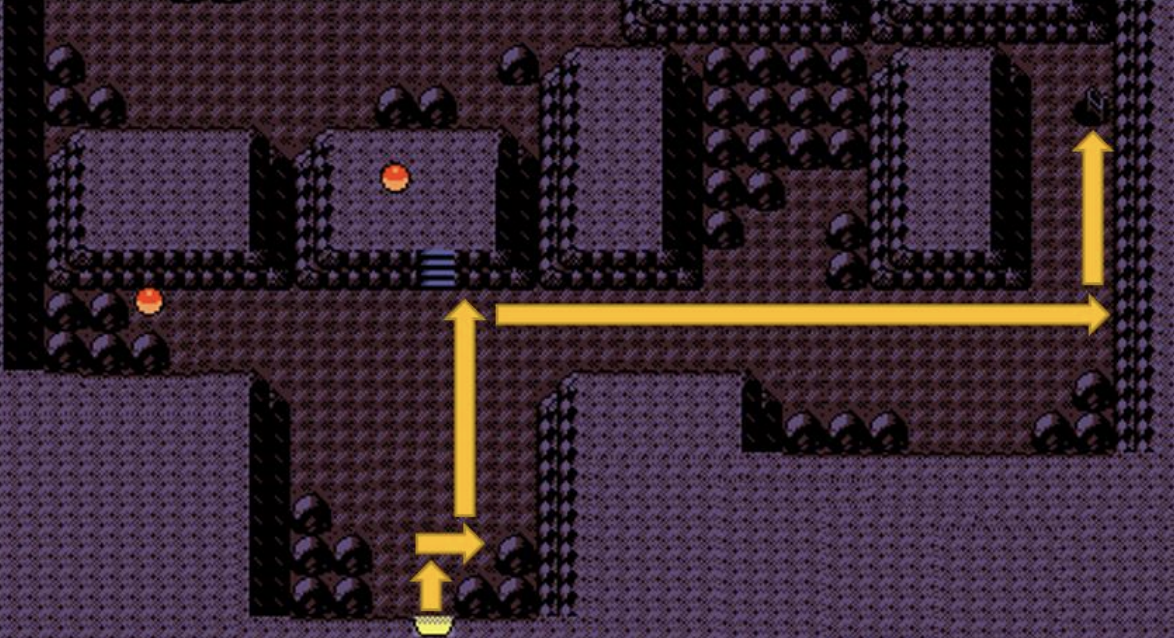
\includegraphics[scale=0.6]{../Graphics/19. Rock Tunnel 1.png}
	\varwe
\end{story}

\begin{story}{Rock Tunnel Path \#3}
	\varwb
	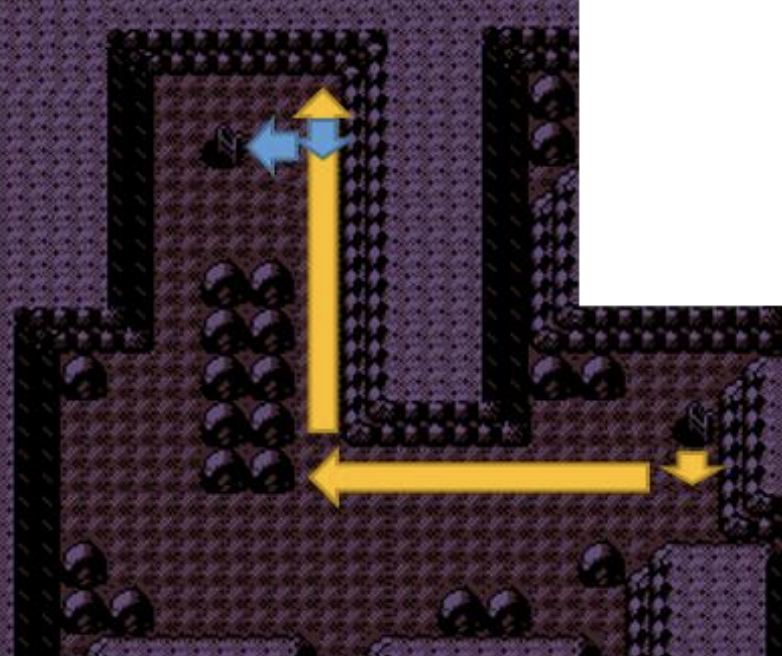
\includegraphics[scale=0.3]{../Graphics/21. Rock Tunnel 3.png}
	\varwe
\end{story}

\begin{story}{Rock Tunnel Path \#5}
	\varwb
	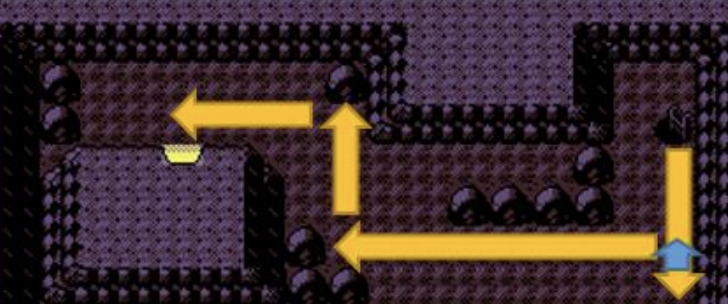
\includegraphics[scale=0.75]{../Graphics/23. Rock Tunnel 5.png}
	\varwe
\end{story}

\switchcolumn
\vspace{4.9cm}
\begin{story}{Rock Tunnel Path \#2}
	\varwb
	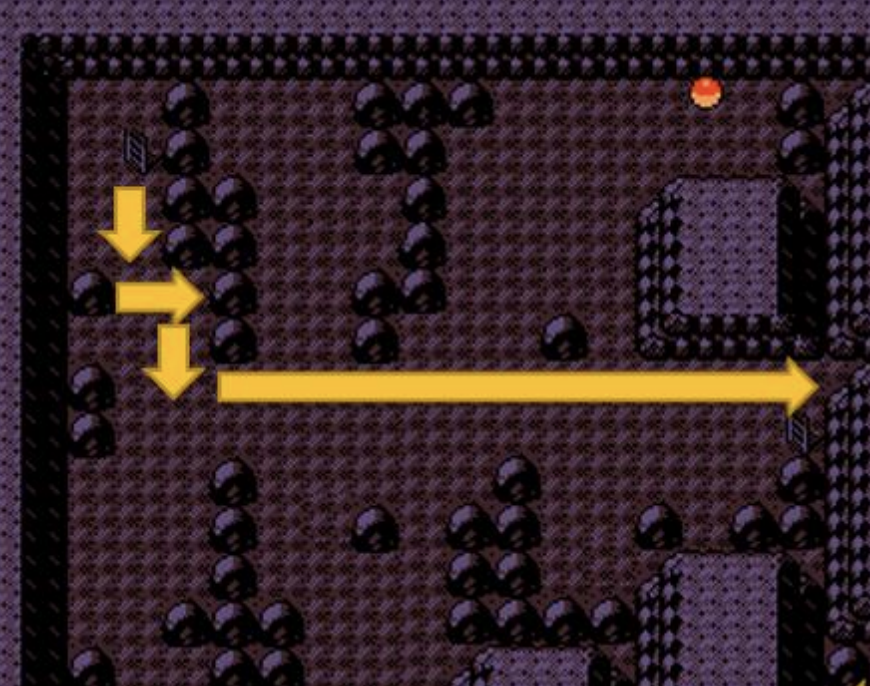
\includegraphics[scale=0.5]{../Graphics/20. Rock Tunnel 2.png}
	\varwe
\end{story}

\newpage
\begin{story}{Rock Tunnel Path \#4}
	\varwb
	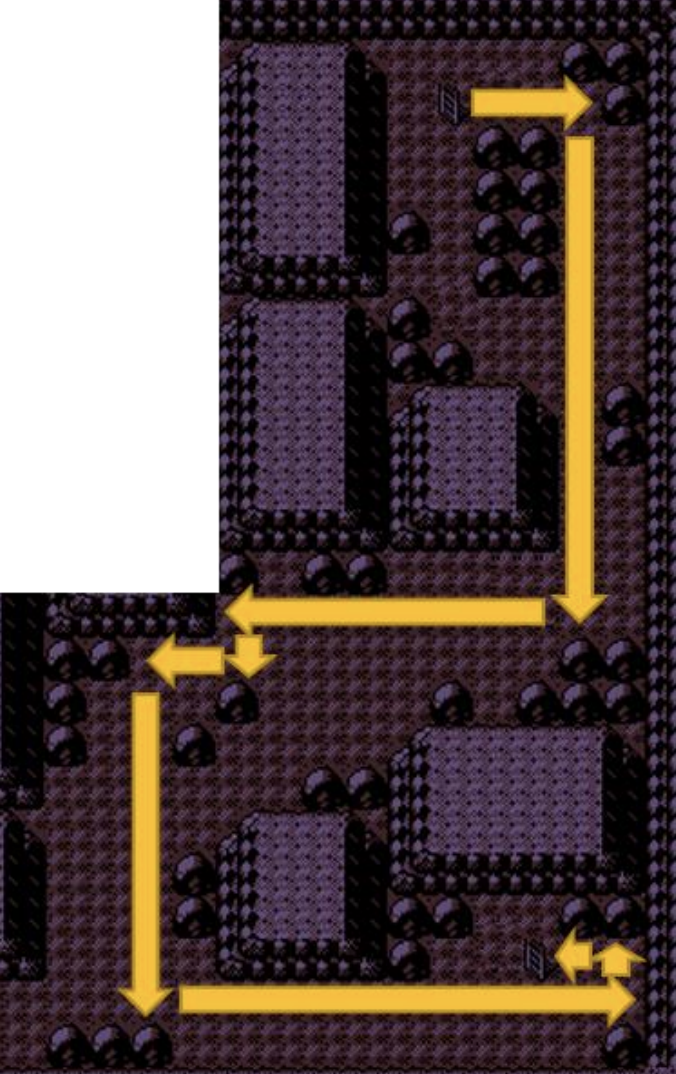
\includegraphics[scale=0.35]{../Graphics/22. Rock Tunnel 4.png}
	\varwe
\end{story}

\switchcolumn
\begin{enumerate}[resume]
	\item After leaving the Rock Tunnel, \emphasis{enter and exit the Pokemon Center}
	\item Head north to the water's edge and then east
	\item Surf south and exit on the patch of grass to enter the Power Plant
	\item Head northeast and down to \dialog{talk to the man in red}
\end{enumerate} 

\switchcolumn
\begin{story}{Fly to Saffron City}
	\varwb
	\insertMap{../Graphics/24. Saffron City.png}
	\varwe
\end{story}

\switchcolumn
\begin{menu}{After Exiting the Power Plant}
	\varwb
	\begin{pokeMenu}
		\item \menuHlTwo{(1)} \fly{} to Saffron City \menuHlTwo{(\pointDown)}
	\end{pokeMenu}
	\varwe
\end{menu}

\begin{enumerate}[resume]
	\item Exit Saffron City northwest and head northwest to Celadon City
	\item Head southwest \pointRight{} east \pointRight{} Cut the tree to head to the Gym
\end{enumerate} 

\begin{trainer}{Twins Jo \& Zoe}
	\varwb
	\begin{fightSection}{Victreebel/Vileplume}
		\item \trainerHl{(1)} \return{} \trainerHlTwo{2x}
	\end{fightSection}
	\varwe
\end{trainer}

\begin{trainer}{Picnicker Tanya (Left Trainer)}
	\varwb
	\begin{fightSection}{Exeggutor}
		\item \trainerHl{(1)} \return
		\begin{notes}
			\small{\item \trainerHl{(4)} \icePunch{} \textit{(if $<$12 DV ATK)}}
		\end{notes}
	\end{fightSection}
	\varwe
\end{trainer}

\begin{trainer}{Beauty Julia}
	\varwb
	\begin{fightSection}{Paras/Exeggcute/Parasect}
		\item \trainerHl{(2)} \strength{} \trainerHlTwo{3x}
	\end{fightSection}
	\varwe
\end{trainer}

\begin{boss}{Erika}
	\varwb
	\begin{fightSection}{Tangela}
		\item \bossHl{(4)} \icePunch
	\end{fightSection}
	\begin{fightSection}{Jumpluff}
		\item \bossHl{(1)} \return
	\end{fightSection}
	\begin{fightSection}{Victreebel}
		\item \xAttack
		\item \bossHl{(1)} \return
	\end{fightSection}
	\begin{fightSection}{Bellossom}
		\item \bossHl{(1)} \return
	\end{fightSection}
	\varwe
\end{boss}

\switchcolumn*
\vspace{-3.55cm}
\begin{story}{Fly to Saffron City}
	\varwb
	\insertMap{../Graphics/24. Saffron City.png}
	\varwe
\end{story}

\switchcolumn
\begin{menu}{After Exiting the Gym}
	\varwb
	\begin{pokeMenu}
		\item \menuHlTwo{(1)} \fly{} to Saffron City \menuHlTwo{(\pointDown)}
	\end{pokeMenu}
	\varwe
\end{menu}

\end{paracol}
\vspace{3.5mm} 
\chapter{Marsh and Cascade Badges}
\vspace{0.5mm}

\begin{paracol}{2}
\begin{enumerate}
	\item Follow the path right and up (all the way) to the Gym
	\item \emphasis{Avoid spinner: Medium Rebecca} and take the top-right teleporter
	\item Left \pointRight{} down \emphasis{(left against the wall)} \pointRight{} down \emphasis{(left against the wall)}
\end{enumerate}

\switchcolumn
\vspace{0.8cm}
\begin{trainer}{Medium Rebecca}
	\varwb
	\begin{fightSection}{Drowzee/Hypno}
		\item \trainerHl{(1)} \return{} \trainerHlTwo{2x}
	\end{fightSection}
	\varwe
\end{trainer}

\switchcolumn
\begin{boss}{Sabrina}
	\varwb
	\begin{fightSection}{Espeon/Mr. Mime/Alakazam}
		\item \bossHl{(1)} \return{} \bossHlTwo{3x}
	\end{fightSection}
	\varwe
\end{boss}

\begin{enumerate}[resume]
	\item Exit the Gym: leave Sabrina \pointRight{} right \pointRight{} up \pointRight{} up \pointRight{} down
	\item Exit Saffron through the north gate
	\item Take the northeast path and follow it to the Gym (under the wood fence)
	\item Exit the gym \pointRight{} back southeast the wood fence \pointRight{} head northwest to the bridge
	\item Start heading east down Route 24
\end{enumerate}

\begin{trainer}{Schoolboy Dudley}
	\varwb
	\begin{fightSection}{Oddish}
		\item \trainerHl{(2)} \strength
	\end{fightSection}
	\varwe
\end{trainer}

\begin{trainer}{Lass Ellen}
	\varwb
	\begin{fightSection}{Wigglytuff/Granbull}
		\item \trainerHl{(3)} \surf{} \trainerHlTwo{2x}
	\end{fightSection}
	\varwe
\end{trainer}

\begin{trainer}{Schoolboy Joe}
	\varwb
	\begin{fightSection}{Tangela/Vaporeon}
		\item \trainerHl{(1)} \return{} \trainerHlTwo{2x}
	\end{fightSection}
	\varwe
\end{trainer}

\switchcolumn*
\vspace{2.3cm}
\begin{misc}{When You Hit L58}
	\varwb
	\begin{notes}
		\item \emphasis{B \pointRight{} A to cancel learning Hydro Pump}
	\end{notes}
	\varwe
\end{misc}

\switchcolumn
\begin{trainer}{Lass Laura}
	\varwb
	\begin{fightSection}{Gloom/Bellossom/Pidgeotto}
		\item \trainerHl{(2)} \strength{} \trainerHlTwo{3x}
	\end{fightSection}
	\varwe
\end{trainer}

\begin{trainer}{Camper Lloyd}
	\varwb
	\begin{fightSection}{Nidoking}
		\item \trainerHl{(1)} \return
	\end{fightSection}
	\varwe
\end{trainer}

\begin{trainer}{Lass Shannon}
	\varwb
	\begin{fightSection}{Paras/Paras/Parasect}
		\item \trainerHl{(2)} \strength{} \trainerHlTwo{3x}
	\end{fightSection}
	\varwe
\end{trainer}

\begin{trainer}{Super Nerd Pat}
	\varwb
	\begin{fightSection}{Porygon}
		\item \trainerHl{(1)} \return
	\end{fightSection}
	\varwe
\end{trainer}

\switchcolumn*
\begin{story}{Fly to Cerulean City}
	\varwb
	\insertMap{../Graphics/25. Cerulean City.png}
	\varwe
\end{story}

\switchcolumn
\begin{menu}{After Interrupting Misty}
	\varwb
	\begin{pokeMenu}
		\item \menuHlTwo{(1)} \fly{} to Cerulean City \menuHlTwo{(\pointUp)}
	\end{pokeMenu}
	\varwe
\end{menu}

\begin{enumerate}[resume]
	\item Head east to the Gym
	\item Walk up the east wall and Surf to Misty
\end{enumerate}

\begin{boss}{Misty}
	\varwb
	\begin{fightSection}{Golduck}
		\item \bossHl{(1)} \return
	\end{fightSection}
	\begin{fightSection}{Quagsire}
		\item \xAttack
		\item \bossHl{(1)} \return
	\end{fightSection}
	\begin{fightSection}{Lapras/Starmie}
		\item \bossHl{(1)} \return
		\begin{notes}
			\small{\item \bossHl{(2)} \strength{} \textit{(if necessary)}}
		\end{notes}
	\end{fightSection}
	\varwe
\end{boss}

\switchcolumn
\begin{items}{Hidden Machine Part}
	\varwb
	\insertScreenshot{../Graphics/26. Machine Part.png}
	\varwe
\end{items}

\switchcolumn
\begin{enumerate}[resume]
	\item Grab the hidden \pickup{Machine Part} on the way out
\end{enumerate}

\begin{menu}{After Exiting the Gym}
	\varwb
	\begin{packMenu}
		\item \superRepel
	\end{packMenu}
	\begin{pokeMenu}
		\item \menuHlTwo{(1)} \teleport
	\end{pokeMenu}
	\varwe
\end{menu}

\end{paracol}
\vspace{3.5mm} 
\chapter{Thunder and Boulder Badges}
\vspace{0.5mm}

\begin{paracol}{2}
\begin{enumerate}
	\item Head north and Surf around to the Power Plant
	\item Head inside and \dialog{talk to the man in red on the right side again}
\end{enumerate}

\switchcolumn
\begin{story}{Fly to Lavender Town}
	\varwb
	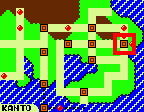
\includegraphics[scale=1.0125]{../Graphics/27. Lavender Town.png}
	\varwe
\end{story}

\switchcolumn
\begin{menu}{After Exiting the Power Plant}
	\varwb
	\begin{pokeMenu} 
		\item \menuHlTwo{(1)} \fly{} to Lavender Town \menuHlTwo{(3\pointDown)}
	\end{pokeMenu}
	\varwe
\end{menu}

\begin{enumerate}[resume]
	\item Head east to the Radio Tower and \dialog{get the Expn Card from the man in the top-right}
\end{enumerate}

\switchcolumn
\begin{story}{Fly to Vermilion City}
	\varwb
	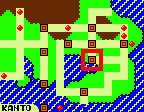
\includegraphics[scale=1.0125]{../Graphics/18. Vermilion City.png}
	\varwe
\end{story}

\switchcolumn
\begin{menu}{After Exiting the Radio Tower}
	\varwb
	\begin{pokeMenu} 
		\item \menuHlTwo{(1)} \fly{} to Vermilion City \menuHlTwo{(2\pointUp)}
	\end{pokeMenu}
	\varwe
\end{menu}

\begin{enumerate}[resume]
	\item Head southwest to the Gym and fight the trainer on the right
\end{enumerate}

\begin{trainer}{Gentleman Gregory}
	\varwb
	\begin{fightSection}{Pikachu/Flaaffy}
		\item \trainerHl{(4)} \icePunch{} \trainerHlTwo{2x}
	\end{fightSection}
	\varwe
\end{trainer}

\begin{boss}{Lt. Surge}
	\varwb
	\begin{fightSection}{Raichu/Magneton}
		\item \bossHl{(3)} \surf{} \bossHlTwo{2x}
	\end{fightSection}
	\begin{fightSection}{Electabuzz}
		\item \bossHl{(1)} \return
	\end{fightSection}
	\begin{fightSection}{Electrode/Electrode}
		\item \bossHl{(2)} \strength{} \bossHlTwo{2x}
	\end{fightSection}
	\varwe
\end{boss}

\begin{enumerate}[resume]
	\item Exit and bike east out of Vermilion City to Snorlax
\end{enumerate}

\begin{menu}{At Snorlax}
	\varwb
	\begin{packMenu} 
		\item \superRepel
	\end{packMenu}
	\begin{gearMenu}
		\item \textbf{Radio \menuHlTwo{(3)}} \pointRight{} tune to 20 \menuHlTwo{(\pointUp)}
	\end{gearMenu}
	\varwe
\end{menu}

\begin{enumerate}[resume]
	\item Run from Snorlax and make your way through Diglett's Cave
	\item Head west and Cut the tree
	\item \emphasis{Go around the trainer in the grass} and head northwest and around into the Gym
\end{enumerate}

\begin{trainer}{Camper Jerry}
	\varwb
	\begin{fightSection}{Sandslash}
		\item \trainerHl{(1)} \return
		\begin{notes}
			\small{\item \trainerHl{(4)} \icePunch{} \textit{(if $<$13 DV ATK)}}
		\end{notes}
	\end{fightSection}
	\varwe
\end{trainer}

\begin{boss}{Brock}
	\varwb
	\begin{fightSection}{Graveler/Kabutops/Omastar/Onix/Rhyhorn}
		\item \bossHl{(3)} \surf{} \bossHlTwo{5x}
	\end{fightSection}
	\varwe
\end{boss}

\end{paracol}
\vspace{3.5mm} 
\chapter{Volcano and Soul Badges}
\vspace{0.5mm}

\begin{paracol}{2}
\begin{enumerate}
	\item Head north back around the Gym and head south
	\item \emphasis{Head around the trainer through the grass and head southwest}
	\item Go through the maze and get the hidden \pickup{Max Ether} before continuing
\end{enumerate}

\switchcolumn
\begin{items}{Hidden Max Ether}
	\varwb
	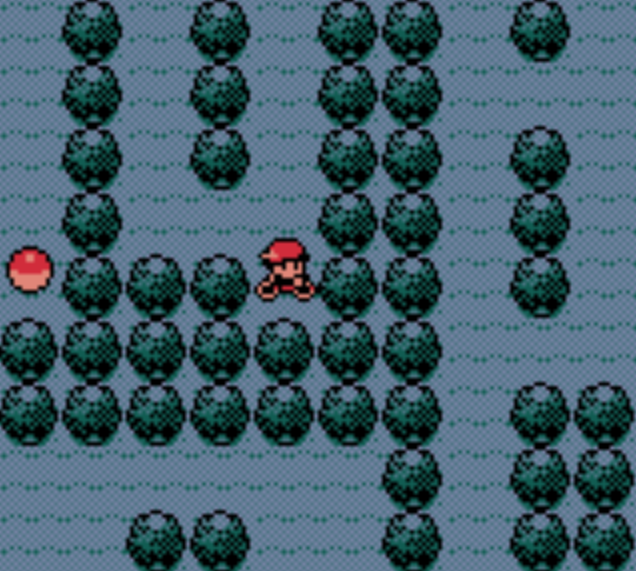
\includegraphics[scale=0.2525]{../Graphics/28. Hidden Max Ether.png}
	\varwe
\end{items}

\switchcolumn
\resume
\begin{enumerate}[resume]
	\item After exiting \emphasis{go one tile left} before heading down
	\item Continue south to Pallet Town 
\end{enumerate}

\begin{menu}{Before the Grass}
	\varwb
	\begin{packMenu}
		\item \maxEther{} \pointRight{} \return{} \menuHlTwo{(1)}
		\item \maxRepel
	\end{packMenu}
	\varwe
\end{menu}

\begin{enumerate}[resume]
	\item Surf south \emphasis{(stick to the left wall)} to Cinnabar Island and \dialog{talk to Blue}
	\item Go southeast near the Pokemon Center and Surf east
	\item \emphasis{Swim north along the coast and then east to stay above the platform}
	\item After the platform continue east until Seafoam Island
	\item Enter the cave to fight Blaine
\end{enumerate}

\begin{boss}{Blaine}
	\varwb
	\begin{fightSection}{Magcargo}
		\item \bossHl{(3)} \surf
	\end{fightSection}
	\begin{fightSection}{Magmar}
		\item \bossHl{(1)} \return
	\end{fightSection}
	\begin{fightSection}{Rapidash}
		\item \bossHl{(3)} \surf
	\end{fightSection}
	\varwe
\end{boss}

\begin{enumerate}[resume]
	\item Exit the cave and Surf to the north wall
	\item Continue east and north to the land
	\item Bike north and continue to the Fuchsia City Gym
	\item Head up on the right side and make your way to the bottom-left trainer
\end{enumerate}

\begin{boss}{Janine}
	\varwb
	\begin{fightSection}{Crobat/Ariados/Weezing/Weezing/Venomoth}
		\item \bossHl{(1)} \return{} \bossHlTwo{5x}
	\end{fightSection}
	\varwe
\end{boss}

\switchcolumn*
\vspace{-3.55cm}
\begin{story}{Fly to Viridian City}
	\varwb
	\insertMap{../Graphics/29. Viridian City.png}
	\varwe
\end{story}

\switchcolumn
\begin{menu}{After Exiting the Gym}
	\varwb
	\begin{pokeMenu}
		\item \menuHlTwo{(1)} \fly{} to Viridian City \menuHlTwo{(2\pointUp)}
	\end{pokeMenu}
	\varwe
\end{menu}

\end{paracol}
\vspace{3.5mm} 
\chapter{Blue and Red}
\vspace{0.5mm}

\begin{paracol}{2}
\begin{enumerate}
	\item Bike north (all the way up) \pointRight{} east \pointRight{} around the back of the Gym to enter
\end{enumerate}

\begin{boss}{Blue}
	\varwb
	\begin{fightSection}{Pidgeot}
		\item \xAttack{} \bossHlTwo{2x}
		\begin{notes}
			\item \bossNote{\textbf{3x} if $<$11 DV ATK}
		\end{notes}
		\item \bossNote{\xSpeed{} if $<$11 DV SPD}
		\item \bossHl{(1)} \return
	\end{fightSection}
	\begin{fightSection}{Exeggutor/Alakazam/Gyarados/Arcanine}
		\item \bossHl{(1)} \return{} \bossHlTwo{4x}
	\end{fightSection}
	\begin{fightSection}{Rhydon}
		\item \bossHl{(3)} \surf
	\end{fightSection}
	\varwe
\end{boss}

\switchcolumn
\vspace{2.48cm}
\begin{story}{Fly to Pallet Town}
	\varwb
	\insertMap{../Graphics/30. Pallet Town.png}
	\varwe
\end{story}

\switchcolumn
\begin{menu}{After Exiting the Gym}
	\varwb
	\begin{pokeMenu}
		\item \menuHlTwo{(1)} \fly{} to Pallet Town \menuHlTwo{(\pointUp)}
	\end{pokeMenu}
	\varwe
\end{menu}

\begin{enumerate}[resume]
	\item Head southeast to the Lab to \dialog{speak to Professor Oak}
\end{enumerate}

\switchcolumn
\begin{story}{Fly to Viridian City}
	\varwb
	\insertMap{../Graphics/29. Viridian City.png}
	\varwe
\end{story}

\switchcolumn
\begin{menu}{After Exiting the Lab}
	\varwb
	\begin{packMenu}
		\item \maxRepel
	\end{packMenu}
	\begin{pokeMenu}
		\item \menuHlTwo{(1)} \fly{} to Viridian City \menuHlTwo{(2\pointUp)}
	\end{pokeMenu}
	\varwe
\end{menu}

\begin{enumerate}[resume]
	\item Bike northwest to the checkpoint and take the west exit
	\item Continue west (south side) and then north into Mt. Silver
	\item Follow the image to get through it
\end{enumerate}

\switchcolumn
\begin{story}{Mt. Silver Path}
	\varwb
	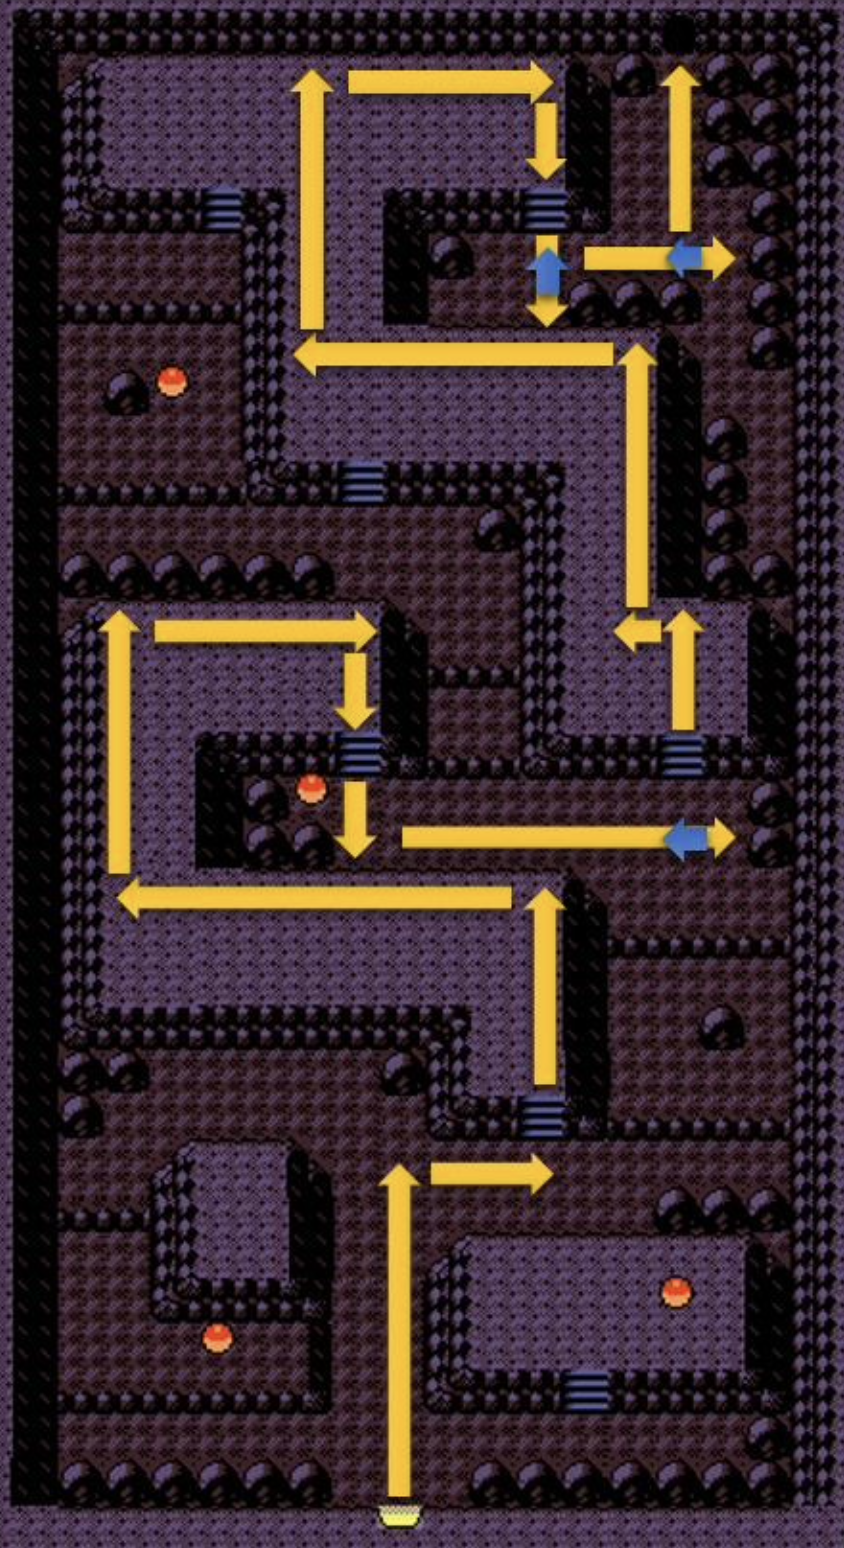
\includegraphics[scale=0.45]{../Graphics/31. Mt. Silver.png}
	\varwe
\end{story}

\switchcolumn
\begin{menu}{When Repel Runs Out}
	\varwb
	\begin{packMenu}
		\item \maxRepel
		\item \fullRestore
	\end{packMenu}
	\varwe
\end{menu}

\begin{boss}{Red}
	\varwb
	\begin{fightSection}{Pikachu}
		\item \bossNote{\fullRestore{} if \textbf{\thunder} hits anytime}
		\item \guardSpec
		\item \xAttack{} \bossHlTwo{2x}
		\begin{notes}
			\item \bossNote{\textbf{3x} if $<$11 DV ATK}
		\end{notes}
		\item \xSpeed
		\item \bossHl{(1)} \return
	\end{fightSection}
	\begin{fightSection}{Venusaur/Espeon/Snorlax/Blastoise/Charizard}
		\item \bossHl{(1)} \return
	\end{fightSection}
	\varwe
\end{boss}

\end{paracol}
\vspace{3.5mm} 

%----------end of document----------%
\end{document}
